% !TEX root = FDS_Technical_Reference_Guide.tex

\chapter{Nomenclature}
\label{nomenclature}

\begin{tabbing}
$A_s$ \hspace{1in}        \= droplet surface area \\
$A_{\alpha\beta}$          \> pre-exponential factor for solid phase Arrhenius reaction \\
$B$                       \> pre-exponential factor for gas phase Arrhenius reaction \\
$C$                       \> Sprinkler C-Factor \\
$C_D$                     \> drag coefficient \\
$C_s$                     \> Smagorinsky constant (LES)  \\
$c_s$                     \> Solid material specific heat \\
$c_p$                     \> constant pressure specific heat \\
$D$                       \> diffusion coefficient   \\
$d_m$                     \> median volumetric droplet diameter \\
$E$                       \> activation energy \\
$\bof_b$                  \> external force vector (excluding gravity) \\
$g$                       \> acceleration of gravity \\
$\bg$                     \> gravity vector, normally $(0,0,-g)$ \\
$\cal H$                  \> total pressure divided by the density \\
$H_{r,\alpha\beta}$       \> heat of reaction for a solid phase reaction \\
$h$                       \> enthalpy; heat transfer coefficient   \\
$h_\alpha$                \> enthalpy of species $\alpha$   \\
$h_\alpha^0$              \> heat of formation of species $\alpha$   \\
$I$                       \> radiation intensity   \\
$I_b$                     \> radiation blackbody intensity   \\
$k$                       \> thermal conductivity; suppression decay factor \\
$\dm_{b,\alpha}'''$       \> mass production rate of species $\alpha$ by evaporating droplets/particles \\
$\dm_f''$                 \> fuel mass flux \\
$\dm_\alpha'''$           \> mass production rate of species $\alpha$ per unit volume \\
$\dm_w''$                 \> water mass flux  \\
$m_w''$                   \> water mass per unit area \\
$\NU$                     \> Nusselt number \\
$\PR$                     \> Prandtl number \\
$p$                       \> pressure \\
$\bp_0$                   \> atmospheric pressure profile \\
$\bp_m$                   \> background pressure of $m$th pressure zone \\
$\tp$                     \> pressure perturbation \\
$\dbq''$                  \> heat flux vector \\
$\dq'''$                  \> heat release rate per unit volume \\
$\dq_r''$                 \> radiative flux to a solid surface \\
$\dq_c''$                 \> convective flux to a solid surface \\
$\dQ$                     \> total heat release rate \\
$Q^*$                     \> characteristic fire size \\
$\R$                      \> universal gas constant \\
$\RE$                     \> Reynolds number \\
$r_d$                     \> droplet radius \\
$r_{\alpha\beta}$         \> solid phase reaction rate \\
$\hbox{RTI}$              \> Response Time Index of sprinkler \\
$\bs$                     \> unit vector in direction of radiation intensity\\
$\SC$                     \> Schmidt number \\
$\SH$                     \> Sherwood number \\
$S_\alpha$                \> solid component production rate \\
$T$                       \> temperature \\
$t$                       \> time           \\
$U$                       \> integrated radiant intensity \\
$\bu=(u,v,w)$             \> velocity vector  \\
$W_\alpha$                \> molecular weight of gas species $\alpha$ \\
$\bW$                     \> molecular weight of the gas mixture \\
$\WE$                     \> Weber number \\
$\bx=(x,y,z)$             \> position vector  \\
$X_\alpha$                \> volume fraction of species $\alpha$   \\
$Y_\alpha$                \> mass fraction of species $\alpha$   \\
$\bar{Y}_\alpha$          \> mean mass fraction of species $\alpha$   \\
$\hat{Y}_\alpha$          \> mass fraction of species $\alpha$ in mixed zone of a computation cell   \\
$Y_\OTWO^\infty$          \> mass fraction of oxygen in the ambient   \\
$Y_\F^I$                  \> mass fraction of fuel in the fuel stream   \\
$y_s$                     \> soot yield \\
$Z$                       \> mixture fraction   \\
$Z_f$                     \> stoichiometric value of the mixture fraction   \\
$\gamma$                  \> ratio of specific heats; Rosin-Rammler exponent \\
$\Delta H$                \> heat of combustion \\
$\Delta H_\OTWO$          \> energy released per unit mass oxygen consumed \\
$\delta$                  \> wall thickness \\
$\epsilon$                \> dissipation rate \\
$\kappa$                  \> absorption coefficient \\
$\mu$                     \> dynamic viscosity \\
$\nu_\alpha$              \> stoichiometric coefficient, species $\alpha$ \\
$\nu_s$                   \> yield of solid residue in solid phase reaction \\
$\nu_g,\gamma$            \> yield of gaseous species $\gamma$ in solid phase reaction \\
$\rho$                    \> density \\
$\btau_{ij}$              \> viscous stress tensor \\
$\chi_r$                  \> radiative loss fraction \\
$\sigma$                  \> Stefan-Boltzmann constant; constant in droplet size distribution; surface tension \\
$\sigma_d$                \> droplet scattering coefficient \\
$\sigma_s$                \> scattering coefficient \\
$\bo=(\omx,\omy,\omz)$    \> vorticity vector \\
\end{tabbing}





\chapter{A Velocity Divergence Constraint for Large-Eddy Simulation of Low-Mach Flows}
\label{app_divergence}

The equations governing the evolution of a low-Mach, variable density flows---first introduced by Rehm and Baum in 1978 \cite{Rehm:1}---are continuity, species concentration (mass fraction), momentum, energy (sensible enthalpy), and the ideal gas equation of state:
\begin{gather}
\label{eqn_rho} \frac{\partial \rho}{\partial t} + \Div(\rho\mathbf{u}) = 0 \\
\label{eqn_Y_a} \frac{\partial \rho Y_\alpha}{\partial t} + \Div(\rho Y_\alpha \mathbf{u}) = \Div (\rho D_\alpha \nabla Y_\alpha) + \dot{m}_\alpha^\tripleprime \\
\label{eqn_u}   \frac{\partial \rho \mathbf{u}}{\partial t} + \Div(\rho \mathbf{u} \mathbf{u}) = -\nabla \tilde{p} - \Div\underline{\underline{\tau}} + (\rho-\rho_0) \mathbf{g} \\
\label{eqn_h_s} \frac{\partial \rho h_s}{\partial t} + \Div(\rho h_s \mathbf{u}) = \frac{\mbox{D} \bar{p}}{\mbox{D} t} + \dot{q}^\tripleprime - \Div \dot{\mathbf{q}}^\pp \\
\label{eqn_eos} \rho = \frac{\bar{p} \overline{W}}{RT}
\end{gather}

In this appendix, starting from the conservative form of the sensible enthalpy transport equation, we derive a numerically consistent velocity divergence constraint for use in large-eddy simulation (LES) of low-Mach flows.  The result accounts for numerical transport of mass and energy, which is difficult to eliminate in relatively coarse, engineering LES calculations when total variation diminishing (TVD) scalar transport schemes are employed.  Without the correction terms derived here, unresolved (numerical) mixing of gas species with different heat capacities or molecular weights may lead to erroneous mixture temperatures and ultimately to an imbalance in the energy budget.

\section*{The Divergence Constraint}
\label{div_constraint}

As mentioned, the present work stems from attempts to understand and correct an energy budget imbalance which became evident after implementing both temperature-dependent specific heats and TVD scalar transport. One of the revelations of this work has been that the choice of starting point for deriving the divergence constraint naturally leads to two different forms of the divergence expression.  While these forms are mathematically equivalent, they lead to two completely different---and yet completely plausible---numerical formulations.

\subsection*{From Continuity}
Starting from the continuity equation, we can factor out the velocity divergence leaving the material derivative of the density:
\begin{align}
\Div\mathbf{u} &= -\frac{1}{\rho}\frac{\D\rho}{\D t}
\end{align}
Using the ideal gas law and differentiating the equation of state leads to
\begin{align}
\label{eqn_div_1}
\Div\mathbf{u} &= \left(\frac{1}{\rho c_p T} - \frac{1}{\bar{p}} \right)\frac{\mbox{D} \bar{p}}{\mbox{D} t} \notag\\
&+ \frac{1}{\rho c_p T} \left[ \dot{q}^\tripleprime - \Div \dot{\mathbf{q}}^\pp \right] \notag\\
&+ \frac{1}{\rho} \sum_\alpha \left(\frac{\overline{W}}{W_\alpha} - \frac{h_{s,\alpha}}{c_p T} \right) \left[ \Div (\rho D_\alpha \nabla Y_\alpha) + \dot{m}_\alpha^\tripleprime \right]
\end{align}

\subsection*{From Sensible Enthalpy}
Alternatively, we may factor the velocity divergence from the sensible enthalpy transport equation:
\begin{align}
\label{eqn_div_new}
\Div\mathbf{u} &= \frac{1}{\rho h_s} \left[ \frac{\D}{\D t}(\bar{p}-\rho h_s) + \dot{q}^\tripleprime - \Div \dot{\mathbf{q}}^\pp \right]
\end{align}
From this starting point, (arguably) the natural result for the divergence expression is
\begin{align}
\label{eqn_div_2}
\Div\mathbf{u} &= \frac{1}{\rho c_p T}\frac{\mbox{D} \bar{p}}{\mbox{D} t} - \frac{1}{\bar{p}} \frac{\partial \bar{p}}{\partial t} \notag\\
&+ \frac{1}{\rho c_p T}\left[ \dot{q}^\tripleprime - \Div \dot{\mathbf{q}}^\pp - \mathbf{u} \cdot\nabla (\rho h_s) \right] \notag\\
&+ \frac{1}{\rho} \sum_\alpha \left(\frac{\overline{W}}{W_\alpha} - \frac{h_{s,\alpha}}{c_p T} \right) \bigg[ \Div (\rho D_\alpha \nabla Y_\alpha) - \mathbf{u} \cdot \nabla (\rho Y_\alpha) + \dot{m}_\alpha^\tripleprime\bigg]
\end{align}

\subsection*{Comparison}
Notice the subtle differences between the first, second, and third lines of (\ref{eqn_div_1}) and (\ref{eqn_div_2}).  The first lines differ by $\displaystyle (\mathbf{u}\cdot\nabla \bar{p})/\bar{p}$. In (\ref{eqn_div_2}), the second and third lines each contain an extra term accounting for advection of enthalpy and mass, respectively, $\mathbf{u} \cdot\nabla (\rho h_s)$ and $\mathbf{u} \cdot \nabla (\rho Y_\alpha)$.  Using (\ref{eqn_rho})-(\ref{eqn_eos}), it can be shown that (\ref{eqn_div_1}) and (\ref{eqn_div_2}) are mathematically equivalent (see Section \ref{equivalence}).


%% CHECK THAT THIS IS CORRECT BEFORE UNCOMMENTING

%\paragraph{Simplifications for Constant Specific Heat} Recall that for an ideal gas we may write
%\begin{align}
%c_{p,\alpha} = c_{v,\alpha} + R/W_\alpha = \frac{R}{W_\alpha} \left(\frac{\gamma_\alpha}{\gamma_\alpha-1}\right) \,\mbox{,}
%\end{align}
%where $c_{p,\alpha}$ is the specific heat of $\alpha$ at constant pressure, $c_{v,\alpha}$ is the specific heat at constant volume, and $\gamma_\alpha = c_{p,\alpha}/c_{v,\alpha}$.  Commonly, the ratio of specific heats is approximated to be constant, and for fire calculations typically the value for air is chosen, $\gamma \approx 1.4$.  In this case, the sensible enthalpy becomes
%\begin{align}
%\rho h_s = \rho c_p T = \rho T \sum_\alpha Y_\alpha c_{p,\alpha} = \rho R T \left(\frac{\gamma}{\gamma-1}\right)\sum_\alpha \frac{Y_\alpha}{W_\alpha} = \rho \frac{R T}{\overline{W}} \left(\frac{\gamma}{\gamma-1}\right) = \bar{p}\left(\frac{\gamma}{\gamma-1}\right)
%\end{align}

\subsection*{The Discrete Divergence}
\label{discrete_divergence}

The \emph{conservative form} of the sensible enthalpy transport equation---which derives its name from the flux divergence form of the mean transport term on the left-hand-side---is
\begin{equation}
\label{eqn_conservative_enthalpy}
\frac{\partial (\rho h_s)}{\partial t} + \underbrace{\Div(\rho h_s \mathbf{u})}_{\mbox{mean transport}} = \frac{\D \bar{p}}{\D t} + \dot{q}^\tripleprime - \Div \dot{\mathbf{q}}^\pp \,\mbox{.}
\end{equation}
This form is called conservative because, by Gauss's theorem, the integral of the discrete flux divergence over the domain is equivalent to the surface integral of the flux over the boundary of the domain.  For a periodic domain the integral is zero---\emph{flow in} must equal \emph{flow out}. The key to guaranteeing discrete conservation of sensible enthalpy is to first discretize the mean transport term.  Below an overline will denote a slope-limiting interpolation operator.  As discussed in Section \ref{app_transport_decomposition}, this operator is specially designed to be consistent with flux-limited, total variation diminishing (TVD) transport for the conservative form of the mean transport term.

Expanding the mean transport term and rearranging (\ref{eqn_conservative_enthalpy}) in terms of the discrete divergence yields
\begin{equation}
\label{eqn_discrete_divergence}
\Div \mathbf{u} = \frac{1}{\rho h_s}\left[ -\left( \frac{\partial (\rho h_s)}{\partial t} + \overline{\mathbf{u}\cdot\nabla(\rho h_s)} \right) + \frac{\D \bar{p}}{\D t} + \dot{q}^\tripleprime - \Div \dot{\mathbf{q}}^\pp \right] \,\mbox{.}
\end{equation}
The numerical details of $\overline{\mathbf{u}\cdot\nabla(\rho h_s)}$ are the key to assuring discrete conservation (see Section \ref{app_transport_decomposition}). Mathematically, (\ref{eqn_discrete_divergence}) is  equivalent to (\ref{eqn_div_new}). Numerically, however, (\ref{eqn_discrete_divergence}) accounts for the critical details of the TVD transport scheme.

Most of the complexity in the divergence expression is buried in the time derivative term, $\partial (\rho h_s)/\partial t$.  Using (\ref{eqn_rho})-(\ref{eqn_eos}), it can be shown that (\ref{eqn_discrete_divergence}) expands to yield (\ref{eqn_div_2}) (see Appendix \ref{app_time_derivative}).


\section*{Factoring the Discrete Flux Divergence}
\label{app_transport_decomposition}

Below we show the numerical decomposition of the enthalpy flux divergence for cell $i$ in 1D.  The operator $\delta(\,\,\,)/\delta x$ denotes a central difference.  Density $\rho$ and sensible enthalpy $h_s$ are stored at cell centers indexed by $i$, $i+1$, etc.  Velocity $u$ is stored at the cell face and indexed by $i+\mhalf$, etc.  Here an overline applied to a face value ($i\pm\mhalf$ suffix) denotes a flux limiter, which is basically a special interpolation of the scalar field to the cell face.  The purpose of the flux limiter is to prevent spurious oscillations in the scalar solution.  Such oscillations must be avoided because they may lead to boundedness violations and instability.

In decomposing the flux divergence, our goal is to break the term into two parts as follows:
\begin{align}
\label{eqn_flux_decomposition}
\left[\frac{\delta (\rho h_s u)}{\delta x}\right]_i &= \frac{ \overline{(\rho h_s)}_{i+\thalf} u_{i+\thalf} - \overline{(\rho h_s)}_{i-\thalf} u_{i-\thalf} }{\delta x} \notag\\
&= (\rho h_s)_i \underbrace{\frac{u_{i+\thalf}-u_{i-\thalf}}{\delta x}}_{\displaystyle\Div\mathbf{u}} + \underbrace{\frac{\Delta_{i+\thalf} u_{i+\thalf} + \Delta_{i-\thalf} u_{i-\thalf}}{\delta x}}_{\displaystyle\overline{\mathbf{u}\cdot\nabla(\rho h_s)}}
\end{align}
Here $\Delta_{i+\thalf}$ represents a limited slope of the scalar data ($\rho h_s$ in this case) at the face $i+\frac{1}{2}$.  The slope limiters for cell $i$ are defined such that
\begin{align}
\label{eqn_slope_1} (\rho h_s)_i + \Delta_{i+\thalf} = \overline{(\rho h_s)}_{i+\thalf} \\
\label{eqn_slope_2} (\rho h_s)_i - \Delta_{i-\thalf} = \overline{(\rho h_s)}_{i-\thalf}
\end{align}

Note that while scalar face values are unique to the face $\left[\overline{(\rho h_s)}_{i+\thalf} = \overline{(\rho h_s)}_{i+1-\thalf}\right]$, the limited slopes are not ($\Delta_{i+\thalf} \ne \Delta_{i+1-\thalf}$).

\subsection*{Example: Pure Upwinding}
Suppose all $u>0$ in 1D, a wind from left to right.  For Godunov's scheme (first-order upwinding) the limited slopes would be computed as follows:
\begin{align}
\Delta_{i+\thalf} &= \overline{(\rho h_s)}_{i+\thalf} - (\rho h_s)_i \notag\\
&= (\rho h_s)_i - (\rho h_s)_i \notag\\
&= 0
\end{align}
\begin{align}
\Delta_{i-\thalf} &= (\rho h_s)_i - \overline{(\rho h_s)}_{i-\thalf} \notag\\
&= (\rho h_s)_i - (\rho h_s)_{i-1}
\end{align}
The cell-average advection term therefore becomes
\begin{align}
\overline{\mathbf{u}\cdot\nabla(\rho h_s)} &= u_{i-\thalf} \left[ \frac{(\rho h_s)_i - (\rho h_s)_{i-1}}{\delta x} \right]
\end{align}

\subsection*{Example: Central Differencing}
For central differencing the limited slopes would be computed as follows:
\begin{align}
\Delta_{i+\thalf} &= \overline{(\rho h_s)}_{i+\thalf} - (\rho h_s)_i \notag\\
&= \frac{1}{2}\left[(\rho h_s)_i + (\rho h_s)_{i+1}\right] - (\rho h_s)_i \notag\\
&= \frac{1}{2}\left[(\rho h_s)_{i+1} - (\rho h_s)_i\right]
\end{align}
\begin{align}
\Delta_{i-\thalf} &= (\rho h_s)_i - \overline{(\rho h_s)}_{i-\thalf} \notag\\
&= (\rho h_s)_i - \frac{1}{2}\left[(\rho h_s)_{i-1} + (\rho h_s)_i\right] \notag\\
&= \frac{1}{2}\left[ (\rho h_s)_i - (\rho h_s)_{i-1} \right]
\end{align}
The cell-average advection term therefore becomes
\begin{align}
\overline{\mathbf{u}\cdot\nabla(\rho h_s)} &= \frac{1}{2}  u_{i+\thalf} \left[ \frac{(\rho h_s)_{i+1} - (\rho h_s)_i}{\delta x} \right] + \frac{1}{2} u_{i-\thalf} \left[ \frac{(\rho h_s)_i - (\rho h_s)_{i-1}}{\delta x} \right]
\end{align}

\subsection*{General Implementation: Using Flux Limiters}
The examples above are for illustration purposes only.  In general, we first compute the flux-limited face values and obtain the limited slopes from (\ref{eqn_slope_1}) and (\ref{eqn_slope_2}).  The cell-average advection term is then computed from the second underbrace in (\ref{eqn_flux_decomposition}).


\section*{Decomposing the Time Derivative}
\label{app_time_derivative}

Using the ideal gas law, the time derivative of the enthalpy can be decomposed as follows:
\begin{align}
\label{eqn_drhdt}
\frac{\partial (\rho h_s)}{\partial t} &= \rho \frac{\partial h_s}{\partial t} + h_s \frac{\partial \rho}{\partial t} \notag\\
&= \rho \sum_\alpha \left( Y_\alpha c_{p,\alpha} \frac{\partial T}{\partial t} + h_{s,\alpha} \frac{\partial Y_\alpha}{\partial t}\right) + h_s \frac{\partial \rho}{\partial t} \notag\\
&= \rho c_p \frac{\partial T}{\partial t} + \rho \sum_\alpha h_{s,\alpha} \frac{\partial Y_\alpha}{\partial t} + h_s \frac{\partial \rho}{\partial t} \notag\\
&= \rho c_p T \left[ \frac{1}{\bar{p}} \frac{\partial \bar{p}}{\partial t} + \frac{1}{\overline{W}} \frac{\partial \overline{W}}{\partial t} - \frac{1}{\rho} \frac{\partial \rho}{\partial t}\right] + \rho \sum_\alpha h_{s,\alpha} \frac{\partial Y_\alpha}{\partial t} + h_s \frac{\partial \rho}{\partial t} \notag\\
&= \rho c_p T \left[ \frac{1}{\bar{p}} \frac{\partial \bar{p}}{\partial t} - \sum_\alpha \frac{\overline{W}}{W_\alpha} \frac{\partial Y_\alpha}{\partial t} - \frac{1}{\rho} \frac{\partial \rho}{\partial t}\right] + \rho \sum_\alpha h_{s,\alpha} \frac{\partial Y_\alpha}{\partial t} + h_s \frac{\partial \rho}{\partial t} \notag\\
&=  \frac{\rho c_p T}{\bar{p}} \frac{\partial \bar{p}}{\partial t}  + \rho \sum_\alpha \left( h_{s,\alpha} - c_p T \frac{\overline{W}}{W_\alpha}\right)\frac{\partial Y_\alpha}{\partial t} + (h_s - c_p T) \frac{\partial \rho}{\partial t}
\end{align}
The time derivative of the mass fractions, which originates from the species transport equation, is:
\begin{align}
\label{eqn_dydt}
\frac{\partial Y_\alpha}{\partial t} &= \frac{1}{\rho} \left[ \Div (\rho D_\alpha \nabla Y_\alpha) + \dot{m}_\alpha^\tripleprime - Y_\alpha \frac{\partial \rho}{\partial t} - \Div (\rho Y_\alpha \mathbf{u}) \right]
\end{align}
Using (\ref{eqn_dydt}) in (\ref{eqn_drhdt}) and summing over species to eliminate the density time derivative we obtain
\begin{align}
\label{eqn_drhdt2}
\frac{\partial (\rho h_s)}{\partial t} &= \frac{\rho c_p T}{\bar{p}} \frac{\partial \bar{p}}{\partial t}  + \sum_\alpha \left( h_{s,\alpha} - c_p T \frac{\overline{W}}{W_\alpha}\right)\left[ \Div (\rho D_\alpha \nabla Y_\alpha) + \dot{m}_\alpha^\tripleprime - \mathbf{u}\cdot\nabla(\rho Y_\alpha) - \rho Y_\alpha \Div \mathbf{u} \right]
\end{align}
Plugging (\ref{eqn_drhdt2}) into (\ref{eqn_div_new}) yields (almost done)
%\begin{align}
%\label{eqn_div_3}
%\Div \mathbf{u} &= \frac{1}{\rho h_s}\frac{\mbox{D} \bar{p}}{\mbox{D} t} - \frac{c_p T}{h_s}\frac{1}{\bar{p}} \frac{\partial \bar{p}}{\partial t} \notag\\
%&+ \frac{1}{\rho h_s}\left[ \dot{q}^\tripleprime - \Div \dot{\mathbf{q}}^\pp - \mathbf{u} \cdot\nabla (\rho h_s) \right] \notag\\
%&+ \frac{1}{\rho h_s} \sum_\alpha \left(c_p T\frac{\overline{W}}{W_\alpha} - h_{s,\alpha} \right) \bigg[ \Div (\rho D_\alpha \nabla Y_\alpha) - \mathbf{u} \cdot \nabla (\rho Y_\alpha) - \rho Y_\alpha \Div \mathbf{u} \bigg] \notag\\
%&+ \frac{1}{\rho h_s} \sum_\alpha \left(c_p T\frac{\overline{W}}{W_\alpha} - h_{s,\alpha} \right) \dot{m}_\alpha^\tripleprime
%\end{align}
\begin{align}
\label{eqn_div_4}
\Div \mathbf{u} + \frac{1}{\rho h_s} \sum_\alpha \left(c_p T\frac{\overline{W}}{W_\alpha} - h_{s,\alpha} \right) \rho Y_\alpha \Div \mathbf{u}  &= \frac{1}{\rho h_s}\frac{\mbox{D} \bar{p}}{\mbox{D} t} - \frac{c_p T}{h_s}\frac{1}{\bar{p}} \frac{\partial \bar{p}}{\partial t} \notag\\
&+ \frac{1}{\rho h_s}\left[ \dot{q}^\tripleprime - \Div \dot{\mathbf{q}}^\pp - \mathbf{u} \cdot\nabla (\rho h_s) \right] \notag\\
&+ \frac{1}{\rho h_s} \sum_\alpha \left(c_p T\frac{\overline{W}}{W_\alpha} - h_{s,\alpha} \right) \bigg[ \Div (\rho D_\alpha \nabla Y_\alpha) - \mathbf{u} \cdot \nabla (\rho Y_\alpha) + \dot{m}_\alpha^\tripleprime\bigg]
\end{align}
\begin{align}
\label{eqn_div_5}
\Div \mathbf{u} + \left(\frac{c_p T}{h_s} - 1\right)\Div \mathbf{u}  &= \frac{1}{\rho h_s}\frac{\mbox{D} \bar{p}}{\mbox{D} t} - \frac{c_p T}{h_s}\frac{1}{\bar{p}} \frac{\partial \bar{p}}{\partial t} \notag\\
&+ \frac{1}{\rho h_s}\left[ \dot{q}^\tripleprime - \Div \dot{\mathbf{q}}^\pp - \mathbf{u} \cdot\nabla (\rho h_s) \right] \notag\\
&+ \frac{1}{\rho h_s} \sum_\alpha \left(c_p T\frac{\overline{W}}{W_\alpha} - h_{s,\alpha} \right) \bigg[ \Div (\rho D_\alpha \nabla Y_\alpha) - \mathbf{u} \cdot \nabla (\rho Y_\alpha) + \dot{m}_\alpha^\tripleprime \bigg]
\end{align}
Finally... (compare with (\ref{eqn_div_2}))
\begin{align}
\label{eqn_div_6}
\Div \mathbf{u} &= \frac{1}{\rho c_p T}\frac{\mbox{D} \bar{p}}{\mbox{D} t} - \frac{1}{\bar{p}} \frac{\partial \bar{p}}{\partial t} \notag\\
&+ \frac{1}{\rho c_p T}\left[ \dot{q}^\tripleprime - \Div \dot{\mathbf{q}}^\pp - \mathbf{u} \cdot\nabla (\rho h_s) \right] \notag\\
&+ \frac{1}{\rho} \sum_\alpha \left(\frac{\overline{W}}{W_\alpha} - \frac{h_{s,\alpha}}{c_p T} \right) \bigg[ \Div (\rho D_\alpha \nabla Y_\alpha) - \mathbf{u} \cdot \nabla (\rho Y_\alpha) + \dot{m}_\alpha^\tripleprime \bigg]
\end{align}

\section*{Equivalence between Divergence Expressions}
\label{equivalence}

The equivalence between (\ref{eqn_div_1}) and (\ref{eqn_div_2}) is apparent based on the following:
\begin{flalign}
-\frac{1}{\rho c_p T} \mathbf{u}\cdot\nabla(\rho h_s) - \frac{1}{\rho} \sum_\alpha \left( \frac{\overline{W}}{W_\alpha} - \frac{h_{s,\alpha}}{c_p T} \right) \mathbf{u}\cdot\nabla(\rho Y_\alpha) &&\notag
\end{flalign}
\vskip-\baselineskip
\begin{align}
&= -\frac{1}{\rho c_p T} \left[ \rho \mathbf{u}\cdot\nabla h_s + h_s \mathbf{u}\cdot\nabla \rho \right] - \frac{1}{\rho} \sum_\alpha \left( \frac{\overline{W}}{W_\alpha} - \frac{h_{s,\alpha}}{c_p T} \right) \left[ \rho \mathbf{u}\cdot\nabla Y_\alpha + Y_\alpha \mathbf{u}\cdot\nabla \rho \right] \notag\\
&= -\frac{1}{c_p T} \mathbf{u}\cdot \sum_\alpha \left[ Y_\alpha \nabla h_{s,\alpha} + h_{s,\alpha} \nabla Y_\alpha \right] - \frac{1}{\rho} \mathbf{u}\cdot\nabla \rho - \sum_\alpha \left( \frac{\overline{W}}{W_\alpha} - \frac{h_{s,\alpha}}{c_p T} \right) \mathbf{u}\cdot\nabla Y_\alpha \notag\\
&= -\frac{1}{c_p T} \mathbf{u}\cdot \sum_\alpha Y_\alpha \nabla h_{s,\alpha} - \frac{1}{\rho} \mathbf{u}\cdot\nabla \rho - \sum_\alpha \frac{\overline{W}}{W_\alpha} \mathbf{u}\cdot\nabla Y_\alpha \notag\\
&= -\frac{1}{c_p T} \mathbf{u}\cdot \sum_\alpha Y_\alpha c_{p,\alpha} \nabla T - \frac{1}{\rho} \mathbf{u}\cdot\nabla \rho - \mathbf{u}\cdot \sum_\alpha \overline{W} \nabla (Y_\alpha/W_\alpha) \notag\\
&= -\mathbf{u}\cdot \left[\frac{1}{T} \nabla T + \frac{1}{\rho} \nabla \rho + \overline{W} \nabla (1/\overline{W}) \right] \notag\\
&= -\frac{1}{\bar{p}} \mathbf{u}\cdot \nabla \bar{p}
\end{align}

\chapter{Multi-environment Extension of Reactor Model}

\label{multi_env_edc}

In the current formulation of the reactor model FDS does not transport the mixing variable. At the start of a time step, mixing is assumed to be in the unmixed state. We would like to extend the reactor model so that we can eventually construct PDFs of reactor concentration. The difficulty is how to construct/transport the necessary information to build the PDF.

One efficient way to describe a PDF is to use moments; where a moment can be thought of a statistical descriptor of the distribution. The first moment of a distribution is the mean of the distribution, the second is the variance, etc. Therefore, the more moments we know, the better the description of the distribution we have. For a given PDF, p(y), the $k^{th}$ moment of $y$ of the distribution is:
\begin{equation}\label{eq:int_moment}
_{y}M_{k} = \int y^{k}p(y)\mathrm{d}y
\end{equation}
Solving this integral equation can become difficult as it requires the function form of the PDF. An alternative way to compute moments is to use Gaussian-quadrature, which represents the moment integral in Eq.~\ref{eq:int_moment} as an n-point sum \cite{mcgraw:1997}:
\begin{equation}\label{eq:qmom}
_{y}M_{k}=\displaystyle \sum_{i=1}^{n} \hat y_{i}^{k} w_{i}
\end{equation}
This technique is known as the quadrature method of moments (QMOM) where  $\hat y_i^k$ is known at the $i^{th}$ quadrature point, $w_i$ is known as the $i^{th}$ quadrature weight, and $n$ is the number of quadrature points. If we consider the unmixed fraction as a weight describing the amount of mixing, the steps to obtain higher order statistics about the batch reactor composition begin to take shape. The unmixed fraction, $\zeta$, exists in two probabilistic states: $p1$ and $p2$, where $p2 = 1-p1$. State 1 ($p1$) describes the amount of the cell that is mixed while state 2 ($p2$) describes the unmixed portion. If we know the mass fractions of species in both mixing states (quadrature points) and the corresponding weights to those states, then we can use QMOM to construct the reactor distribution.

In this case, the quadrature weights become the unmixed fraction, $\zeta_{i}$, and the quadrature points become the mass fractions $\phi_{\alpha,i}$. Applying Eq.~\ref{eq:qmom}, the moments of the distribution in the reactor are:
\begin{eqnarray}\label{eq:moments}
M_{0} &=& \displaystyle \sum_{i=1}^{n} \zeta_{i} \\
\nonumber M_{1} &=& \displaystyle \sum_{i=1}^{n} \zeta_{i} \phi_{\alpha,i} \\
\nonumber M_{2} &=& \displaystyle \sum_{i=1}^{n} \zeta_{i} \phi_{\alpha,i}^2
\end{eqnarray}
The mean of the distribution becomes $M_{1}$ and the centered variance becomes $M_{2}-M_{1}^{2}$. To implement subgrid statistics in FDS, we would either need to transport the unmixed fraction or develop a model for the subgrid variance. Since scalar transport is expensive, a first approach is to develop a model to approximate the subgrid variance. If the variance is known, QMOM can then be used to solve for the initial unmixed fraction.


\chapter{A Simple Model of Flame Extinction}

\subsubsection{Frederick W. Mowrer, Department of Fire Protection Engineering, University of Maryland}

\label{mowrer_model}


A diffusion flame immersed in a vitiated atmosphere will extinguish before consuming all the
available oxygen from the atmosphere.  The classic example of this behavior is a candle burning
within an inverted jar.  This same concept has been applied within FDS
to determine the conditions under which the local ambient oxygen concentration will no longer
support a diffusion flame.  In this appendix, the critical adiabatic flame temperature
concept is used to estimate the local ambient oxygen concentration at which extinction will
occur.

Consider a control volume characterized
by a bulk temperature, $T_m$, a mass, $m$, an average specific heat, $\overline{c_p}$, and an oxygen mass
fraction, $Y_\OTWO$.  Complete combustion of the oxygen within the control volume would release a
quantity of energy given by:
\be
   Q = m \, Y_\OTWO \, \left( \frac{\Delta H}{r_\OTWO}  \right)  \label{bbb}
\ee
where $\Delta H/r_\OTWO$ has a relatively constant value of
approximately 13100~kJ/kg for most fuels of interest for fire applications.\footnote{C. Huggett, ``Estimation of the Rate of Heat Release by Means of Oxygen
Consumption,'' {\em Fire and Materials}, Vol.~12, pp.~61-65, 1980.}
Under adiabatic conditions, the energy released by combustion of the available oxygen within
the control volume would raise the bulk temperature of the gases within the control volume by an
amount equal to:
\be
   Q = m \, \overline{c_p} \, (T_f - T_m)  \label{eee}
\ee
The average specific heat of the gases within the control volume can be calculated based on the
composition of the combustion products as:
\be
   \overline{c_p} = \frac{1}{(T_f-T_m)} \, \sum_\alpha \int_{T_m}^{T_f} c_{p,\alpha} (T) \, dT
\ee
To simplify the analysis, the combustion products are assumed to have an average specific heat
of 1.2~kJ/kg/K over the temperature range of interest, a value similar to that of nitrogen, the primary
component of the products.
The relationship between the oxygen mass fraction within the control volume and the adiabatic
temperature rise of the control volume is evaluated by equating Eqs.~(\ref{bbb}) and (\ref{eee}):
\be
   Y_\OTWO = \frac{ \overline{c_p} (T_f-T_m) }{\Delta H/r_\OTWO}
\ee
If the critical adiabatic flame temperature is assumed to have a constant value of approximately
1700~K for hydrocarbon diffusion flames, as suggested by Beyler,\footnote{C. Beyler, ``Flammability Limits of Premixed and Diffusion Flames,''
{\em SFPE Handbook of Fire Protection Engineering} (3rd Ed.), National Fire
Protection Association, Quincy, MA, 2003.} then the relationship
between the limiting oxygen mass fraction and the bulk temperature of a control volume is given
by:
\be
   Y_{\OTWO,lim} = \frac{ \overline{c_p} (T_{f,lim}-T_m) }{\Delta H/r_\OTWO} \approx  \frac{ 1.2 \, (1700-T_m) }{ 13100}  \label{extinction_model}
\ee
For a control volume at a temperature of 300~K, i.e., near room temperature, the limiting oxygen
mass fraction would evaluate to $Y_{\OTWO,lim}=0.128$.  This value is consistent with the measurements
of Morehart, Zukoski and Kubota,\footnote{Morehart, J., Zukoski, E., and Kubota, T., ``Characteristics of Large Diffusion Flames
Burning in a Vitiated Atmosphere,'' {\em Third International Symposium on Fire Safety
Science}, Elsevier Science Publishers, pp.~575-583, 1991.} who measured the oxygen concentration at extinction of flames by dilution of air
with combustion products. They found that flames self-extinguished at oxygen concentrations of 12.4~\% to 14.3~\%. Note that their results
are expressed as volume, not mass, fractions. Beyler's chapter in the SFPE Handbook references other researchers who measured oxygen
concentrations at extinction ranging from 12~\% to 15~\%.

\chapter{Numerical Methods for Integration of Complex Chemistry}

\label{chemistry_integration}

To solve the system of ordinary differential equations used for complex chemistry (e.g., multi-step reactions, reversible reactions), FDS uses a second-order Runge-Kutta (RK2) scheme as the foundation for its numerical integrator.  As discussed below, the scheme is augmented with Richardson extrapolation, which increases the accuracy to fourth-order and provides a means of error control.

Our goal is to integrate the ODE
\begin{equation}
\frac{\d Y}{\d t} = f(Y)
\end{equation}
where $f(Y)$ represents a reaction rate law and $Y$ is a species mass fraction (temperature dependence of the rate law is frozen at the initial condition).  The total time interval is the FDS time step, $\delta t$, and the iteration substep is $\Delta t$. The RK2 scheme is given by
\begin{align}
\label{RK2}
Y^* &= Y^k + \Delta t^k \, f(Y^k) \notag\\
Y^{k+1}   &= \frac{1}{2}\,(Y^k + Y^* + \Delta t^k \, f(Y^*))
\end{align}
Here $k$ is the iteration index.  The number of sub-time intervals is determined by an error controller, as described below. This second-order scheme is an improvement upon the first-order explicit scheme used for simple chemistry. To maintain stability for stiff problems, however, an intractable number of time steps may be required.

\subsection*{Richardson Extrapolation}

To overcome this issue, we use Richardson extrapolation. Richardson extrapolation increases the order of accuracy and provides a means of error control. Suppose you have an exact solution $A$ represented by a numerical approximation using the interval $h$ such that the error, $A-A(h)$, can be represented by a polynomial expansion of $h$. For
two different intervals $h$ and $h/2$ we may write
\begin{equation}\label{eq:h1}
A_1={A(h)} + \underbrace{a_{1}(h) + a_{2}(h)^2 + \mathcal{O}(h^3)}_{\mathcal{O}(h)}
\end{equation}
\begin{equation}\label{eq:h2}
A_2=A\left(\frac{h}{2}\right) + \underbrace{a_{1}\left(\frac{h}{2}\right) + a_{2}\left(\frac{h}{2}\right)^2 + \mathcal{O}(h^3)}_{\mathcal{O}(h)}
\end{equation}
Here the subscript on $A$ represents subdivisions of the time step $h$, where $A_1$ takes $h/1$ steps, $A_2$ takes $h/2$ steps, and so on. The $a_{1}$ terms can be eliminated by subtracting Eq.~(\ref{eq:h1}) from two times Eq.~(\ref{eq:h2}):
\begin{equation}\label{eq:A2}
A=2\,A_2-A_1 = 2\,A\left(\frac{h}{2}\right) - A(h) + \underbrace{a_{2}\left(\frac{h}{2}\right)^2 + \mathcal{O}(h^3)}_{\mathcal{O}(h^2)}
\end{equation}
which results in a solution with a higher order of error.

This same technique is applied to the second-order Runge-Kutta scheme with three sub-intervals: $h$, $h/2$, and $h/4$. Because the RK2 scheme was initially second-order, the three-step Richardson extrapolation gives a fourth-order solution \cite{Moin:2001}:
\begin{equation}\label{eq:A4}
A=\frac{4\,A_4-A_2}{3}  + \mathcal{O}(h^4)
\end{equation}
In Eq.~(\ref{eq:A4}), $A$ represents the time updated value of the species concentrations in the mixed reactor zone, $\hat{Y}_{\alpha}$, as found in Eq.~(\ref{eq:mixed_mass_fraction_sub}).

\subsection*{Error Control}

In addition to increasing the order of the error in the numerical scheme, Richardson extrapolation also provides an estimate of the error value. This estimate is calculated via a Taylor expansion:
\begin{equation}\label{eq:error}
error \approx \frac{1}{15}\left(\frac{4\,A_4-A_2}{3} - \frac{4\,A_2-A_1}{3}\right)
\end{equation}
The time step ($\Delta t_{new}$) required to maintain the specified/acceptable error ($err\_tol$) can be calculated by using the local error ($error$), the current time step ($\Delta t$), and the order of error within the numerical integration scheme, in this case fourth-order:
\begin{equation}\label{eq:dt_new}
\Delta t_{new}=\Delta t \left(\frac{err\_tol}{error}\right)^{1/4}
\end{equation}
Eq.~(\ref{eq:dt_new}) indicates that if the error estimate is large relative to the tolerance, then the new time step decreases; whereas if the error is small, then the new time step increases. This dynamic time stepping scheme improves computational efficiency because it allows the integrator to take the largest time step possible bounded by either the error tolerance or the global simulation time step, thus minimizing the total number of integration steps required.

\subsection*{A Total Variation Scheme for Stiff Chemistry}

The stiffness associated with a flame front is handled by the error controller and variable time stepping discussed above. The scheme discussed in this section automatically detects chemical equilibrium, the explicit integration of which is also a stiff problem.  Even with error control, the numerical solution may exhibit numerical fluctuations between the bounds of the error tolerance.  This is an undesirable condition which often occurs in cases with competing or reversible reactions.

If the values are fluctuating around a fixed value bounded by the error tolerance, the integrator is doing extra work by continuing to calculate every fluctuation within a time step. To minimize the computational expense, a total variation (TV) scheme has been developed. This scheme examines the differences in species mass fractions at four consecutive sub-time steps. Within this four point stencil there are three differences for each species mass fraction. The TV scheme compares the absolute value of the sum of the differences to the sum of the absolute values of the differences.  For a monotonic function, the following condition must hold:
\begin{equation}\label{eq:monotone}
\sum_{i=1}^{4}|Y(i+1)-Y(i)| = |\sum_{i=1}^{4}(Y(i+1)-Y(i))|
\end{equation}
The reader unfamiliar with the concept of ``data variation'' should stop and think about this for a moment.  It says that, regardless of other complexities, the monotonicity constraint (no fluctuations) is sufficient guarantee the condition stated in Eq.~(\ref{eq:monotone}).  The corollary is that if Eq.~(\ref{eq:monotone}) does not hold then we are guaranteed to have some level of fluctuation.

The condition which corresponds to the extreme case of repeating fluctuations between the error tolerance bounds for our four point stencil is
\begin{equation}\label{eq:TV}
\sum_{i=1}^{4}|Y(i+1)-Y(i)| = 3 \, |\sum_{i=1}^{4}(Y(i+1)-Y(i))|
\end{equation}
This is illustrated in Fig.~\ref{fig:TV}, which shows a quantity fluctuating between 0 and 1 about a fixed point.
\begin{figure}
\begin{center}
\scalebox{0.45}{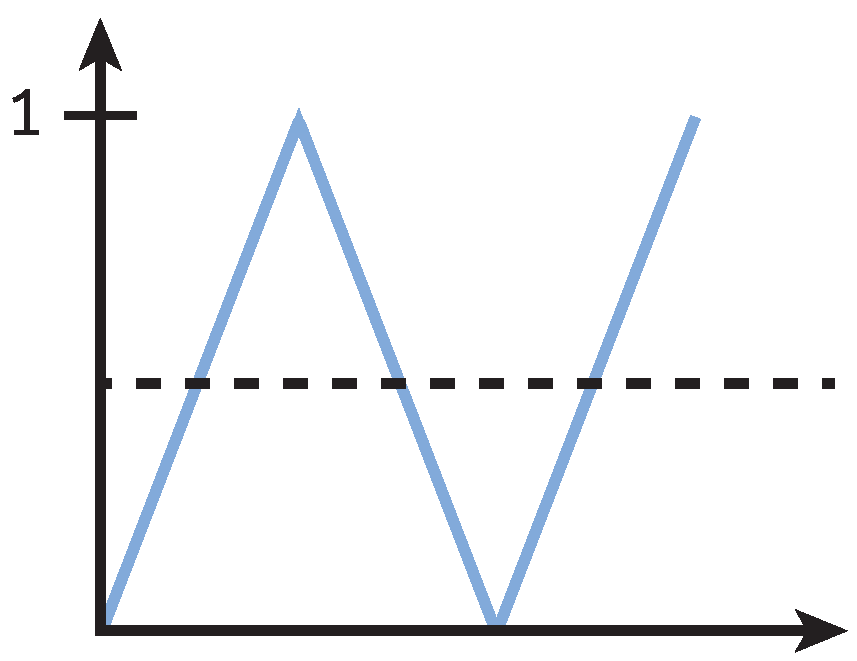
\includegraphics{FIGURES/total_variation}}
\caption{\label{fig:TV} Illustration of a quantity fluctuating between 0 and 1 about a fixed value.}
\end{center}
\end{figure}
We can compare the sum of the absolute value of the differences between the four points,
\begin{equation}\label{eq:sum_abs_tv}
\displaystyle \sum_{i=1}^{4}|Y(i+1)-Y(i)| = |1-0| + |0-1| + |1-0| = 3
\end{equation}
to the absolute value of the sum of the differences,
\begin{equation}\label{eq:abs_sum_tv}
|\displaystyle \sum_{i=1}^{4}(Y(i+1)-Y(i))| = |(1-0)+(0-1)+(1-0)| = 1
\end{equation}
The ratio of Eq.~(\ref{eq:sum_abs_tv}) and Eq.~(\ref{eq:abs_sum_tv}) is 3, which indicates that this data is fluctuating. For the implementation of this scheme in FDS, instead of comparing directly to 3, we use 2.5 because floating point division might not return a value of exactly 3. If fluctuations have been identified, then the values at the fourth point in the stencil are frozen and become the final values at the end of an integration time step. This prevents unnecessary sub-time steps being taken by the integrator. Because the error controller is bounding the solution, any one of the values within the stencil is also within the error tolerance and is therefore acceptable.

%\chapter{Derivation of the Werner Wengle Wall Model}
%%\subsubsection{R. McDermott, BFRL}
%\label{app_WWderivation}
%
%To obtain (\ref{eqn_tauwturb}) we take the first off-wall value of the streamwise velocity to be
%\begin{equation}
%\label{eqn_meanu}
%\tilde{u} = \frac{1}{\Delta z} \int_0^{\Delta z} u(z) \,\mbox{d}z \,\mbox{,}
%\end{equation}
%and then substitute the WW profile for $u(z)$ and integrate.
%
%Let $z_m$ denote the dimensional distance from wall where $z^+ = 11.81$.  Equation (\ref{eqn_meanu}) becomes
%\begin{eqnarray}
%\label{eqn_uint}
%\tilde{u} &=& \frac{1}{\Delta z} \left[ \int_0^{z_m} u(z) \,\mbox{d}z + \int_{z_m}^{\Delta z} u(z) \,\mbox{d}z \right] \,\mbox{,} \nonumber\vspace{0.2cm}\\
%&=& \frac{1}{\Delta z} \left[ \int_0^{z_m} u^+ u^* \,\mbox{d}z + \int_{z_m}^{\Delta z} u^+ u^* \,\mbox{d}z \right] \,\mbox{,} \nonumber\vspace{0.2cm}\\
%&=& \frac{1}{\Delta z} \left[ \int_0^{z_m} z^+ u^* \,\mbox{d}z + \int_{z_m}^{\Delta z} A(z^+)^B u^* \,\mbox{d}z \right] \,\mbox{,} \nonumber\vspace{0.2cm}\\
%&=& \frac{1}{\Delta z} \left[ \int_0^{z_m} \frac{z}{\ell} u^* \,\mbox{d}z + \int_{z_m}^{\Delta z} A\left(\frac{z}{\ell}\right)^B u^* \,\mbox{d}z \right] \,\mbox{,} \nonumber\vspace{0.2cm}\\
%&=& \frac{1}{\Delta z} \left[ \int_0^{z_m} \frac{z\bar{\rho}u^*}{\bar{\mu}} u^* \,\mbox{d}z + \int_{z_m}^{\Delta z} A\left(\frac{z\bar{\rho}u^*}{\bar{\mu}}\right)^B u^* \,\mbox{d}z \right] \,\mbox{,} \nonumber\vspace{0.2cm}\\
%&=& \frac{1}{\Delta z} \left[ \underbrace{\int_0^{z_m} \frac{\tau_w}{\bar{\mu}} z\,\mbox{d}z}_{I} + \underbrace{\int_{z_m}^{\Delta z} A\left(\frac{\bar{\rho}}{\bar{\mu}}\right)^B \left(\frac{\tau_w}{\bar{\rho}}\right)^{\frac{1+B}{2}} z^B\,\mbox{d}z}_{II} \right] \,\mbox{.}
%\end{eqnarray}
%
%We will integrate $I$ and $II$ separately.  First, however, we must find a way to eliminate the unknown $z_m$.  To do this we equate (\ref{eqn_wwlam}) and (\ref{eqn_wwturb}) at the point where the viscous and power law regions intersect, i.e., $z^+ = 11.81 \equiv z_m^+ = z_m \bar{\rho}u^*/\bar{\mu}$.
%\begin{eqnarray}
%\label{eqn_derivezm}
%u^+(z_m^+) = A(z_m^+)^B &=& z_m^+ \nonumber\\
%A &=& (z_m^+)^{1-B} \nonumber\\
%A^{\frac{1}{1-B}} &=& z_m^+ = \frac{z_m\bar{\rho}u^*}{\bar{\mu}} \nonumber\\
%z_m &=& \frac{\bar{\mu}A^{\frac{1}{1-B}}}{\bar{\rho}u^*} \nonumber\\
%z_m &=& \frac{(\bar{\mu}/\bar{\rho})A^{\frac{1}{1-B}}}{\sqrt{\tau_w/\bar{\rho}}} \,\mbox{.}
%\end{eqnarray}
%We now have $z_m$ in terms of $\tau_w$ and otherwise known values.
%
%Integrating section $I$ of (\ref{eqn_uint}) we find
%\begin{eqnarray}
%\label{eqn_intI}
%\int_0^{z_m} \frac{\tau_w}{\bar{\mu}} z\,\mbox{d}z &=& \frac{\tau_w}{2\bar{\mu}} \left[ z^2 \right]_0^{z_m} \nonumber\\
%&=& \frac{\tau_w}{2\bar{\mu}} z_m^2 \nonumber\\
%&=& \frac{\tau_w}{2\bar{\mu}} \frac{(\bar{\mu}/\bar{\rho})^2A^{\frac{2}{1-B}}}{\tau_w/\bar{\rho}} \nonumber\\
%&=& \frac{\bar{\mu} A^{\frac{2}{1-B}}}{2\bar{\rho}} \,\mbox{.}
%\end{eqnarray}
%
%Integrating section $II$ yields
%\begin{eqnarray}
%\label{eqn_intII}
%\int_{z_m}^{\Delta z} A\left(\frac{\bar{\rho}}{\bar{\mu}}\right)^B \left(\frac{\tau_w}{\bar{\rho}}\right)^{\frac{1+B}{2}} z^B\,\mbox{d}z &=& \left\{A\left(\frac{\bar{\rho}}{\bar{\mu}}\right)^B \left(\frac{\tau_w}{\bar{\rho}}\right)^{\frac{1+B}{2}}\right\} \frac{1}{1+B} \left[z^{1+B}\right]_{z_m}^{\Delta z} \nonumber\\
%&=& \left\{ \quad \right\} \frac{1}{1+B} \left[{\Delta z}^{1+B} - {z_m}^{1+B}\right] \nonumber\\
%&=& \left\{ \quad \right\} \frac{1}{1+B} \left[{\Delta z}^{1+B} - \left(\frac{(\bar{\mu}/\bar{\rho})A^{\frac{1}{1-B}}}{\sqrt{\tau_w/\bar{\rho}}}\right)^{1+B}\right] \nonumber\\
%&=& \left\{ \frac{A}{1+B} \left(\frac{\bar{\rho}}{\bar{\mu}}\right)^B \left(\frac{\tau_w}{\bar{\rho}}\right)^{\frac{1+B}{2}} \right\} \left[{\Delta z}^{1+B} - \frac{(\bar{\mu}/\bar{\rho})^{1+B} A^{\frac{1+B}{1-B}}}{\left(\frac{\tau_w}{\bar{\rho}}\right)^{\frac{1+B}{2}}}\right] \nonumber\\
%&=& \frac{A}{1+B} \left(\frac{\bar{\rho}}{\bar{\mu}}\right)^B \left(\frac{\tau_w}{\bar{\rho}}\right)^{\frac{1+B}{2}} {\Delta z}^{1+B} - \frac{(\bar{\mu}/\bar{\rho})}{1+B} A^{\frac{2}{1-B}} \,\mbox{.}
%\end{eqnarray}
%
%Plugging (\ref{eqn_intI}) and (\ref{eqn_intII}) back into (\ref{eqn_uint}) gives
%\begin{eqnarray}
%\label{eqn_combineint}
%\tilde{u} &=& \frac{1}{\Delta z} \left[ \frac{\bar{\mu} A^{\frac{2}{1-B}}}{2\bar{\rho}} + \frac{A}{1+B} \left(\frac{\bar{\rho}}{\bar{\mu}}\right)^B \left(\frac{\tau_w}{\bar{\rho}}\right)^{\frac{1+B}{2}} {\Delta z}^{1+B} - \frac{(\bar{\mu}/\bar{\rho})}{1+B} A^{\frac{2}{1-B}} \right] \nonumber\\
%&=& \frac{1}{2} \left(\frac{\bar{\mu}}{\bar{\rho}\Delta z}\right) A^{\frac{2}{1-B}} - \frac{1}{1+B} \left(\frac{\bar{\mu}}{\bar{\rho}\Delta z}\right) A^{\frac{2}{1-B}} + \frac{A}{1+B} \left(\frac{\bar{\rho}\Delta z}{\bar{\mu}}\right)^B \left(\frac{\tau_w}{\bar{\rho}}\right)^{\frac{1+B}{2}} \,\mbox{.}
%\end{eqnarray}
%Rearranging for $\tau_w$ we find
%\begin{eqnarray}
%\label{eqn_rearrangefortauw}
%\left(\frac{\tau_w}{\bar{\rho}}\right)^{\frac{1+B}{2}} &=& \frac{1+B}{A}\left(\frac{\bar{\mu}}{\bar{\rho}\Delta z}\right)^B \left[ \left( \frac{1}{1+B} - \frac{1}{2}\right)\left(\frac{\bar{\mu}}{\bar{\rho}\Delta z}\right)A^{\frac{2}{1-B}} + \tilde{U} \right] \nonumber\\
%&=& \frac{1-B}{2} A^{\frac{1+B}{1-B}} \left(\frac{\bar{\mu}}{\bar{\rho}\Delta z}\right)^{1+B}  + \frac{1+B}{A} \left(\frac{\bar{\mu}}{\bar{\rho}\Delta z }\right)^B \tilde{U} \nonumber\\
%\tau_w &=& \bar{\rho} \left[ \frac{1-B}{2} A^{\frac{1+B}{1-B}} \left(\frac{\bar{\mu}}{\bar{\rho}\Delta z}\right)^{1+B}  + \frac{1+B}{A} \left(\frac{\bar{\mu}}{\bar{\rho}\Delta z }\right)^B \tilde{u} \right]^{\frac{2}{1+B}} \,\mbox{,}
%\end{eqnarray}
%which corresponds to Eq. (9.46) in \cite{Sagaut:2001}.



\chapter{Scalar Boundedness Correction}
\label{app_boundedness}

Second-order central differencing of the advection term in the scalar transport equation leads to dispersion errors (spurious wiggles) and these errors, if left untreated, can lead to scalar fields which are physically not realizable, e.g., negative densities.  To prevent this, FDS employs a boundedness correction to the scalar fields after the explicit transport step.  The correction, which we describe below, acts locally and effectively adds the minimum amount of diffusion necessary to prevent boundedness violations.  It is stressed that this correction does not make the scalar transport scheme total variation diminishing (TVD); it only serves to correct for boundedness. Similar schemes are employed by others (e.g., \cite{Herrmann:2005}).

By default, FDS employs a TVD transport scheme (Superbee \cite{Roe:1986} for LES and CHARM \cite{Zhou:1995} for DNS). These TVD schemes are applied during the transport step and each can be shown to be TVD in 1D under certain CFL constraints.  However, except for Godunov's scheme ({\ct FLUX\_LIMITER=1}), the TVD proofs do not extend to 3D \cite{Toro}.  Still, these schemes do a much better job than pure central differencing at mitigating dispersion error.  Note that even though TVD schemes are applied, by default FDS still runs through the boundedness check in case any small violations are not prevented by the flux limiter.

\subsubsection{A simple case}

For simplicity we start by considering a minimum boundedness violation for density in 1D.  That is, somewhere we have $\rho < \rho_{min}$.  Let $\rho_i^*$ denote the resulting density from the explicit transport step for cell $i$ with volume $V_i$.  Our goal is to find a correction $\delta \rho_i$ which:
\begin{enumerate}[{(}a{)}]
\item satisfies boundedness, $\rho_i = \rho_i^* + \delta \rho_i \ge \rho_{min}$ for all $i$
\item conserves mass, $\sum_i \delta \rho_i V_i = 0$
\item minimizes data variation, $\sum_i |\delta \rho_i|$ is minimized (i.e., we change the field as little as possible)
\end{enumerate}

As mentioned, the basic idea is to apply a linear smoothing operator $\cal L$ to the density field in regions where boundedness violations have occurred. So, the correction may be viewed as an explicit diffusion step applied to the uncorrected field with diffusion coefficient $c$:
\begin{equation}
\rho = \rho^* + c {\cal L} \rho^*
\end{equation}
To make matters simple, let us envision for the moment that the density in cell $i$ is negative but that the densities in cells $i-1$ and $i+1$ are both safely in bounds (this actually is what happens most of the time with dispersion error).  We therefore want a correction that takes mass away from $i-1$ and $i+1$ and moves it to $i$ to make up the deficit.  We know that for cell $i$ the minimum change in mass and therefore the minimum correction that will satisfy boundedness is $\delta \rho_i = \rho_{min} - \rho_i^*$.  The operator $\cal L$ takes the form of the standard discrete Laplacian.  The correction for cell $i$ is simply
\begin{eqnarray}
\label{eqn_rhocor}
\rho_i &=& \rho_i^* + \delta \rho_i \nonumber\\
&=& \rho_i^* + \rho_{min} - \rho_i^* \nonumber\\
&=&  \rho_i^* + c_i (\rho_{i-1}^* - 2 \rho_i^* + \rho_{i+1}^*)
\end{eqnarray}
Comparing the second and third lines, we find that the diffusion coefficient is given by
\begin{equation}
\label{eqn_diffcoef}
c_i = \frac{\rho_{min} - \rho_i^*}{\rho_{i-1}^* - 2 \rho_i^* + \rho_{i+1}^*}
\end{equation}
Based on the third line of (\ref{eqn_rhocor}), the correction for cell $i$ may be thought of as the sum to two mass fluxes from its neighboring cells.  The change in mass of cell $i$ is $\delta m_i = \delta \rho_i V_i$ and is balanced by changes in mass for cells $i-1$ and $i+1$:
\begin{eqnarray}
\delta m_{i-1} &=& - c_i (\rho_{i-1}^* - \rho_i^*) V_i \nonumber\\
\delta m_{i+1} &=& - c_i (\rho_{i+1}^* - \rho_i^*) V_i \nonumber
\end{eqnarray}
In this case the sum of the mass corrections is zero, as desired:
\begin{eqnarray}
\sum_{j=i-1}^{i+1} \delta m_j &=& \delta \rho_{i-1} V_{i-1} + \delta \rho_i V_i + \delta \rho_{i+1}V_{i+1} \nonumber\\
&=& - c_i (\rho_{i-1}^* - \rho_i^*) V_i + c_i (\rho_{i-1}^* - 2 \rho_i^* + \rho_{i+1}^*) V_i - c_i (\rho_{i+1}^* - \rho_i^*) V_i \nonumber\\
&=& 0 \nonumber
\end{eqnarray}

\subsubsection{Realistic cases}

The discussion above was to provide a simple case for understanding the basic idea behind the correction method.  In a realistic case we must account for multi-dimensional aspects of the problem and for the possibility that neighboring cells may both be out of bounds.  Consider a grid cell whose
density is outside the specified range. Denote this cell with a ``$c$'' for center. Its volume is $V_c$ and density is $\rho_c^*$, obtained from the transport scheme.  Let the subscript ``$n$'' denote any of the six neighboring cells (in other words, only include cells which share a face with cell $c$).  We want to correct any boundedness violations for the  cell $c$ by shifting mass to or from its neighboring cells $n$:
\begin{equation}
\rho_c = \rho_c^* + \delta \rho_c \quad ; \quad \rho_n = \rho_n^* + \delta \rho_n
\end{equation}
We first define the total amount of mass we wish to shift:
\be m_c = | \rho^*_c - \rho_{\rm cut} | \, V_c  \ee
where $\rho_{\rm cut}$ is the appropriate upper or lower bound of the density.
The amount of mass each neighboring cell can accommodate without falling outside the range is:
\be m_n = \Big| \min \Big[ \rho_{\max} , \max[\rho_{\min},\rho_n^*] \Big] - \rho_{\rm cut} \Big| \, V_n \ee
The correction terms that guarantee mass conservation ($V_c \, \delta \rho_c = - \sum V_n \, \delta \rho_n$) are:
\be
\label{eqn_rhomn}
\delta \rho_c = \pm \min \left[ m_c , \sum m_n \right] / V_c  \quad ; \quad
\delta \rho_n = \mp \min \left[ \frac{m_c}{\sum m_n} , 1 \right] m_n/V_n
\ee

Next, to correct species mass fractions that are out of bounds, we follow the exact same procedure.
\begin{equation}
Z_c = Z_c^* + \delta Z_c \quad ; \quad Z_n = Z_n^* + \delta Z_n
\end{equation}
We define the amount of species mass we wish to shift:
\be m_c = | Z^*_c - Z_{\rm cut} | \, \rho_c \, V_c  \ee
where $Z_{\rm cut}$ is either 0 or 1.
The amount of species mass each neighboring cell can accommodate without falling outside the range is:
\be m_n = \Big| \min \Big[ 1 , \max[0,Z_n^*] \Big] - Z_{\rm cut} \Big| \, \rho_n \, V_n \ee
The correction terms that guarantee mass conservation ($V_c \, \rho_c \, \delta Z_c = - \sum V_n \, \rho_n \, \delta Z_n$) are:
\be
\label{eqn_Zmn}
\delta Z_c = \pm \min \left[ m_c , \sum m_n \right] / (\rho_c \, V_c)  \quad ; \quad
\delta Z_n = \mp \min \left[ \frac{m_c}{\sum m_n} , 1 \right] m_n/(\rho_n \, V_n)
\ee


%\subsubsection{An alternate view by R. McDermott}
%
%The discussion above was to provide a simple case for understanding the basic idea behind the correction method.  In a realistic case we must account for multi-dimensional aspects of the problem and for the possibility that neighboring cells may both be out of bounds.  Here again we examine the case of a minimum density boundedness violation. Consider the cell $i$ in a 3D flow with volume $V_i$ and density $\rho_i^*$ obtained from the transport scheme.  Let ${\sf N}$ denote the set of cells containing $i$ and its neighbors, excluding diagonal neighbors (in other words, only include cells which share a face with $i$). We want to correct any boundedness violations for the $i$th cell via
%\begin{equation}
%\rho_i = \rho_i^* + \delta \rho_i
%\end{equation}
%
%To determine $\delta \rho_i$ we must consider the mass exchange between neighboring cells. Let $\delta \rho_{ji}$ denote the density change for cell $j$ in ${\sf N}$ due to a boundedness violation in $i$.  For example, if $\rho_i^* < \rho_{min}$ then the density in $i$ will increase by drawing mass from its neighbors (if the mass is available).  The mass exchange matrix is given by
%\begin{equation}
%\label{eqn_rhoij}
%\delta \rho_{ji} = \left\{ \begin{array}{ll}  \displaystyle \max(0,\rho_{min} - \rho_i^*) & \mbox{if} \quad j=i  \\ \displaystyle -c_i( \max[\rho_{min},\rho_j^*] - \max[\rho_{min},\rho_i^*]) & \mbox{if} \quad j\ne i \end{array} \right.
%\end{equation}
%The smoothing parameter in (\ref{eqn_rhoij}) is obtained from
%\begin{equation}
%\label{eqn_reali}
%c_i = \frac{\max(0,\rho_{min} - \rho_i^*)}{ \sum_{j, j\ne i} ( \max[\rho_{min},\rho_j^*] - \max[\rho_{min},\rho_i^*] )}
%\end{equation}
%
%Mass conservation is obeyed because the mass increase in cell $i$ is balanced by a mass decrease by its neighbors.  In other words, the columns of $\delta \rho_{ji}$ sum to zero.  Note, however, that the mass exchange matrix is not symmetric.  The row sum gives the final mass correction for the $i$th cell:
%\begin{equation}
%\label{eqn_sumdrho}
%\delta \rho_i = \sum_j \delta \rho_{ij}
%\end{equation}



\chapter{The Dynamic Smagorinsky Model}
%\subsubsection{R. McDermott}
\label{app_dynsmag}

The ``subgrid-scale'' (SGS) stress, which accounts for momentum transport by unresolved eddies, emerges from decomposition of the advection term when deriving the LES equations.  It is defined as
\begin{equation}
\label{eqn_tau_sgs}
\tau_{ij}^{sgs} \equiv \bar{\rho}(\widetilde{u_i u_j} - \tilde{u}_i \tilde{u}_j) \,\mbox{.}
\end{equation}
The deviatoric (trace free) part of the SGS stress is modeled by gradient diffusion in analogy with the viscous stress,
\begin{equation}
\label{eqn_tau_sgs_deviatoric}
\tau_{ij}^{sgs} - \frac{1}{3}\tau_{kk}^{sgs} \equiv \tau_{ij}^{sgs,dev} = -2 \mu_t \left(\tilde{S}_{ij} - \frac{1}{3}\tilde{S}_{kk}\delta_{ij}\right) =  -2 \mu_t \left(\tilde{S}_{ij} - \frac{1}{3} (\nabla\!\cdot\tilde{\mathbf{u}}) \delta_{ij}\right) \,\mbox{.}
\end{equation}
In FDS, the turbulent viscosity is obtained from the Smagorinsky model,
\begin{equation}
\label{eqn_mu_turb}
\mu_t = \bar{\rho}(C_s \Delta)^2 |\tilde{S}| \,\mbox{,}
\end{equation}
where $C_s$ is the model constant and $\Delta$ is the filter width taken as the geometric average of the local mesh spacing; for example, in 3D, $\Delta = (\delta x \,\delta y \,\delta z)^{1/3}$.  Note that the quantity $(C_s \Delta)$ is the local ``mixing length'' and that $|\tilde{S}|$ provides the time scale for turbulent diffusion.

In preparation for the dynamic procedure, we rewrite the model for the deviatoric SGS stress as
\begin{equation}
\label{eqn_tau_sgs_deviatoric2}
\tau_{ij}^{sgs,dev} = -2 (C_s \Delta)^2 \beta_{ij} \,\mbox{,}
\end{equation}
defining
\begin{equation}
\label{eqn_beta}
\beta_{ij} = \bar{\rho} |\tilde{S}| \left(\tilde{S}_{ij} - \frac{1}{3} \tilde{S}_{kk} \delta_{ij} \right)  \,\mbox{.}
\end{equation}


\subsubsection{The Dynamic Procedure}

We will now discuss the dynamic procedure for determining $C_s$, the Smagorinsky constant.  The procedure itself is a series of explicit filtering operations leading to a simple algebraic relationship for $C_s(\mathbf{x},t)$ (see Eq.~(\ref{eqn_lengthscale}) below).  The FDS implementation basically follows the works of Germano et al. \cite{Germano:1991}, Moin et al. \cite{Moin:1991}, and Pino Martin et al. \cite{PinoMartin:2000}.

To derive the procedure, first, we apply a ``test'' filter of width $\hat{\Delta}>\Delta$ to the LES equations to obtain
\begin{equation}
\label{eqn_testfiltns}
\frac{\partial \widehat{\overline{\rho u_i}}}{\partial t} + \frac{\partial \widehat{\overline{\rho u_i u_j}}}{\partial x_j} = -\frac{\partial \widehat{\overline{\sigma}}_{ij}}{\partial x_j} \,\mbox{,}
\end{equation}
where $\sigma_{ij}$ is the total stress tensor. The $\,\,\breve{}\,\,$ is adopted from Pino Martin et al.~\cite{PinoMartin:2000} for the Favre test filter, $\widehat{\overline{\rho}} \breve{\widetilde{u}} \equiv \widehat{ \overline{ \rho u }}$, allowing us to rewrite Eq.~(\ref{eqn_testfiltns}) as
\begin{eqnarray}
\label{eqn_testfavrefiltns}
\frac{\partial \widehat{\overline{\rho}} \breve{\widetilde{u}}_i}{\partial t} + \frac{\partial \widehat{\overline{\rho}} \breve{\widetilde{u_i u_j}}}{\partial x_j} &=& -\frac{\partial \widehat{\overline{\sigma}}_{ij}}{\partial x_j} \,\mbox{,} \nonumber\\
\frac{\partial \widehat{\overline{\rho}} \breve{\widetilde{u}}_i}{\partial t} + \frac{\partial \widehat{\overline{\rho}} \breve{\widetilde{u}}_i \breve{\widetilde{u}}_j}{\partial x_j} &=& -\frac{\partial \widehat{\overline{\sigma}}_{ij}}{\partial x_j} - \frac{\partial T_{ij}}{\partial x_j}\,\mbox{,}
\end{eqnarray}
where the ``subtest'' stress is defined as
\begin{equation}
\label{eqn_subteststress}
T_{ij} \equiv \widehat{\overline{\rho}} \left( \breve{\widetilde{u_i u_j}} - \breve{\widetilde{u}}_i \breve{\widetilde{u}}_j \right) \,\mbox{.}
\end{equation}

The deviatoric part of the subtest stress is modeled as,
\begin{equation}
\label{eqn_devtest}
T_{ij} - \frac{1}{3}T_{kk}\delta_{ij} \equiv T_{ij}^{dev} = -2 \left( C_s \widehat{\Delta} \right)^2 \widehat{\overline{\rho}} |\breve{\widetilde{S}}|\left(\breve{\widetilde{S}}_{ij} - \frac{1}{3} \breve{\widetilde{S}}_{kk}\delta_{ij}\right)  \,\mbox{.}
\end{equation}
By applying the Germano identity \cite{Germano:1991}, we obtain the Leonard stress,
\begin{eqnarray}
L_{ij} = T_{ij} - \widehat{\tau_{ij}^{sgs}} &=& \widehat{\overline{\rho}} \left( \breve{\widetilde{u_i u_j}} - \breve{\widetilde{u}}_i \breve{\widetilde{u}}_j \right) - \widehat{ \overline{\rho} \left( \widetilde{u_i u_j} - \widetilde{u}_i \widetilde{u}_j \right)} \,\mbox{,} \nonumber\\
&=&  \widehat{\overline{\rho}} \left( \breve{\widetilde{u_i u_j}} - \breve{\widetilde{u}}_i \breve{\widetilde{u}}_j \right) - \widehat{\overline{\rho}} \left( \breve{\widetilde{u_i u_j}} - \breve{\widetilde{u}_i \widetilde{u}_j} \right) \,\mbox{,} \nonumber \\
\label{eqn_germano} &=&  \widehat{\overline{\rho}} \left( \breve{\widetilde{u}_i \widetilde{u}_j} - \breve{\widetilde{u}}_i \breve{\widetilde{u}}_j \right) \,\mbox{.}
\end{eqnarray}
Using the Favre definitions, Eq.~(\ref{eqn_germano}) may be rearranged to the form typically seen in the literature,
\begin{eqnarray}
L_{ij} &=&  \widehat{\overline{\rho} \frac{\overline{\rho u_i}}{\overline{\rho}} \frac{\overline{\rho u_j}}{\overline{\rho}}} - \widehat{\overline{\rho}} \frac{ \widehat{\overline{\rho u_i}}}{\widehat{\overline{\rho}}} \frac{\widehat{\overline{\rho u_j}}}{\widehat{\overline{\rho}}} \,\mbox{,} \nonumber \\
&=& \widehat{\frac{\overline{\rho u_i}\, \overline{\rho u_j}}{\overline{\rho}}} - \frac{ \widehat{\overline{\rho u_i}} \,\widehat{\overline{\rho u_j}}}{\widehat{\overline{\rho}}} \,\mbox{,} \nonumber \\
\label{eqn_leonard} &=& \widehat{\overline{\rho} \widetilde{u}_i \widetilde{u}}_j - \frac{ \widehat{\overline{\rho} \widetilde{u}}_i \widehat{\overline{\rho} \widetilde{u}}_j }{ \widehat{\overline{\rho}} } \,\mbox{.}
\end{eqnarray}
\LaTeX\,has a hard time covering the entire term with the ``wide'' version of the hat, but please note that the entire first term of Equation \ref{eqn_leonard} is test filtered. The Leonard term is computable from resolved LES values.

If we now look at the \emph{model} for the Germano identity (the deviatoric part) we have,
\begin{equation}
\label{eqn_germanomodel}
L_{ij}^{dev} = T_{ij}^{dev} - \widehat{\tau_{ij}^{sgs,dev}} \approx - 2\left(C_s \widehat{\Delta}\right)^2 \widehat{\overline{\rho}} |\breve{\widetilde{S}}| \left( \breve{\widetilde{S}}_{ij} - \frac{1}{3} \breve{\widetilde{S}}_{kk} \delta_{ij} \right) +  2 \left(C_s \Delta \right)^2 \widehat{\beta}_{ij} \,\mbox{.}
\end{equation}
Note that the entire last term should be test filtered, since $C_s$ is not necessarily uniform.  However, without pulling the length scale out of the filter operation it is difficult to compute a value for $C_s$.

We now rearrange (\ref{eqn_germanomodel}) to facilitate coding,
\begin{equation}
\label{eqn_codemodel}
L_{ij}^{dev} = \left(C_s \Delta\right)^2 M_{ij}^{dev} \,\mbox{,}
\end{equation}
where,
\begin{equation}
\label{eqn_Mij}
M_{ij}^{dev} = 2\left(\widehat{\beta}_{ij} - \alpha \widehat{\overline{\rho}} |\breve{\widetilde{S}}| \left( \breve{\widetilde{S}}_{ij} - \frac{1}{3}\breve{\widetilde{S}}_{kk} \delta_{ij} \right) \right) \,\mbox{,}
\end{equation}
and $\alpha = (\widehat{\Delta}/\Delta)^2$.  For a test filter two times the grid width it appears we should have $\alpha = 4$.  However, as discussed by Lund \cite{Lund:1997}, the method of discrete quadrature significantly affects the results. If using the trapezoid rule, as we do in FDS, then $\alpha = 6$.

We can now compute $L_{ij}$ and $M_{ij}^{dev}$ from known LES quantities.  If we right multiply Eq.~(\ref{eqn_codemodel}) by $M_{ij}^{dev}$, we obtain our desired result:
\begin{equation}
\label{eqn_lengthscale}
\left(C_s \Delta\right)^2 = \frac{ L_{ij}^{dev} M_{ij}^{dev} }{ M_{ij}^{dev} M_{ij}^{dev} } \,\mbox{.}
\end{equation}

\subsubsection{Notes on implementation}

\begin{enumerate}
\item
It is unnecessary to compute the deviatoric part of the Leonard term.  This is because, fortunately, $L_{ij} M_{ij}^{dev} = L_{ij}^{dev} M_{ij}^{dev}$.  Here's the proof (thanks to Stas Borodai of Reaction Engineering International):
\begin{eqnarray}
L_{ij} M_{ij}^{dev} &=& L_{ij} \left( M_{ij} - \frac{1}{3}M_{kk}\delta_{ij} \right) \,\mbox{,} \nonumber \\
&=& L_{ij} M_{ij} - \frac{1}{3} L_{ij}\delta_{ij} M_{kk} \,\mbox{,} \nonumber \\
\label{eqn_LMD} &=& L_{ij} M_{ij} - \frac{1}{3} L_{qq} M_{kk} \,\mbox{.}
\end{eqnarray}
\begin{eqnarray}
L_{ij}^{dev} M_{ij}^{dev} &=& \left( L_{ij} - \frac{1}{3}L_{qq}\delta_{ij} \right) \left( M_{ij} - \frac{1}{3}M_{kk}\delta_{ij} \right) \,\mbox{,} \nonumber \\
&=& L_{ij} M_{ij} - \frac{1}{3} L_{ij}\delta_{ij} M_{kk} - \frac{1}{3} M_{ij}\delta_{ij} L_{qq} + \frac{1}{9} \delta_{ij} \delta_{ij} L_{qq} M_{kk} \,\mbox{,} \nonumber \\
&=& L_{ij} M_{ij} - \frac{1}{3} M_{kk} L_{qq} - \frac{1}{3} L_{qq} M_{kk} + \frac{1}{3} M_{kk} L_{qq} \,\mbox{,} \nonumber \\
\label{eqn_LDMD} &=& L_{ij} M_{ij} - \frac{1}{3} L_{qq} M_{kk} \,\mbox{.}
\end{eqnarray}
Equations (\ref{eqn_LMD}) and (\ref{eqn_LDMD}) are equal and so there is no need to go to the trouble of subtracting the isotropic part out of $L_{ij}$.
\item
The length scale should be averaged over some homogeneous region to maintain stability,
\begin{equation}
\label{eqn_finallengthscale}
\left(C_s \Delta\right)^2 = \frac{ \langle L_{ij} M_{ij}^{dev} \rangle}{ \langle M_{ij}^{dev} M_{ij}^{dev} \rangle } \,\mbox{.}
\end{equation}
In FDS, the brackets denote a spatial average over the test filter width.  If the denominator is zero, the constant is set to zero.
\item
It is common practice to ``clip'' the eddy viscosity.  In theory, a negative value of the eddy viscosity produces backscatter of energy from unresolved to resolved motions.  If this sounds dangerous from a stability perspective, it is.  The simple solution is to set $C_s = 0$, if $\langle L_{ij}M_{ij}^{dev} \rangle < 0$.
\end{enumerate}



\chapter{Fluid-Particle Momentum Transfer}

The trajectories of Lagrangian particles in FDS could be calculated with forward-Euler integration. However, forward-Euler integration extracts momentum from the cell each particle started in. This can cause large changes in the flow field unless the time step is extremely small. An extremely small time step would be necessary for stability. This time step would greatly slow down the calculation. Consequently, a stable, single-step approximate solution is developed and is implemented in FDS.

Two effects are neglected in this formulation. The first is the effect of the change in droplet mass between  time steps. The droplet's evaporation is not coupled to this model. This is justified because the change in droplet mass per time step is small. The second neglected effect is the change in drag coefficient between time steps. This is justified because of the large uncertainties in the drag coefficients. Modeling the time derivative of the drag coefficient will not improve accuracy beyond these uncertainties, but it will slow down the simulation.

\subsubsection{Relative velocities}
Let $m_p$ denote the particle mass, $\mathbf{u}_p$ the particle velocity, $A_p$ the particle cross-sectional area, $C_{\text{d},p}$ the particle drag coefficient, $\rho_\text{a}$ the fluid mass density, $\mathbf{U}_p$ the fluid velocity around the particle, $V_\text{g}$ is the volume occupied by the fluid in a cell, and $M \equiv \rho_\text{a} V_\text{g}$ the fluid mass of a cell, $n_\text{p}$ is the number of particles in a cell, $M_\text{p} \equiv M/n_\text{p}$ is the average fluid mass per particle in a cell, and $\mathbf{g}$ is the gravitational acceleration vector.

The equations of motion of the particles and fluid are formulated as follows from Newton's second law,
\begin{align}
    \label{particle_eom}
    m_p \frac{\text{d} \mathbf{u}_p}{\text{d} t} &= - \frac{1}{2} \rho_\text{a} C_{\text{d},p} A_p (\mathbf{u}_p - \mathbf{U}_p) |\mathbf{u}_p - \mathbf{U}_p| + m_p \mathbf{g} \\
    \label{fluid_eom}
    M_p \frac{\text{d} \mathbf{U}_p}{\text{d} t} &= \frac{1}{2} \rho_\text{a} C_{\text{d},p} A_p (\mathbf{u}_p - \mathbf{U}_p) |\mathbf{u}_p - \mathbf{U}_p| \,.
\end{align}
Note that the fluid Eq. (\ref{fluid_eom}) does not include a gravity term. This gravity term is included in the Navier-Stokes equations; including it here would be redundant. Also note that lift is not included here.

If we define $\mathbf{u}_\text{r} \equiv \mathbf{u}_p - \mathbf{U}_p$ as the relative velocity between the fluid and the particle, we can find a single equation for the relative velocity by dividing both equations by their respective masses (i.e., $m_p$ and $M_p$) and then subtracting the second from the first. This result is
\begin{align}
    \frac{\text{d} \mathbf{u}_\text{r}}{\text{d} t} = -\frac{1}{2} \rho_\text{a} C_{\text{d},p} A_p \left(\frac{1}{m_p} + \frac{1}{M_p} \right) \mathbf{u}_\text{r} |\mathbf{u}_\text{r}| + \mathbf{g} \,.
\end{align}
The equation above can be written in short as
\begin{align}
    \frac{\text{d} \mathbf{u}_\text{r}}{\text{d} t} = -K_p \mathbf{u}_\text{r} |\mathbf{u}_\text{r}| + \mathbf{g} \quad ; \quad K_p \equiv \frac{1}{2} \rho_\text{a} C_{d_p} A_p \left(\frac{1}{m_p} + \frac{1}{M_p} \right) \,.
\end{align}
Note that the $p$ subscripts have been dropped in $\mathbf{u}_\text{r}$ terms for convenience. The $p$ subscript also will be dropped from some other variables later as convenient.

This is the drag equation, which has no solution in terms of elementary functions. Our solution approach first finds a solution neglecting gravity and then adds in a series for the gravity terms. $\mathbf{u}_\text{r} \equiv \mathbf{u}_\text{d} + \mathbf{u}_\text{g}$ is the decomposition of $\mathbf{u}_\text{r}$. $\mathbf{u}_\text{r}$ and $\mathbf{u}_\text{d}$ both have the same initial condition, $\mathbf{u}_\text{r}(0) \equiv \mathbf{u}_p(0) - \mathbf{U}_p(0) = \mathbf{u}_{p,0} - \mathbf{U}_{p,0}$. $\mathbf{u}_\text{d}$ satisfies the drag equation without gravity, specifically
\begin{align}
    \frac{\text{d} \mathbf{u}_\text{d}}{\text{d} t} = -K_p \mathbf{u}_\text{d} |\mathbf{u}_\text{d}| \,.
\end{align}
The solution subject to these initial conditions is
\begin{align}
    \label{ud_exact}
    \mathbf{u}_\text{d} = \frac{\mathbf{u}_{p,0} - \mathbf{U}_{p,0}}{1 + \beta_p t} \quad ; \quad \beta_p \equiv K_p |\mathbf{u}_{\text{r},0}| \,.
\end{align}
We decompose can $u_\text{r}$ to find a series solution for $\mathbf{u}_\text{g}$ with Taylor series. The function $\mathbf{u}_\text{g}$ can be written $\mathbf{u_g} = \mathbf{u}_\text{r} - \mathbf{u}_\text{d}$ so the differential equation for $\mathbf{u}_\text{g}$ is
\begin{align}
    \frac{\text{d} \mathbf{u}_\text{g}}{\text{d} t} = -K_p (\mathbf{u}_\text{r} |\mathbf{u}_\text{r}| - \mathbf{u}_\text{d} |\mathbf{u}_\text{d}|) + \mathbf{g} \quad ; \quad \mathbf{u}_\text{g}(0) = \mathbf{u}_\text{r}(0) - \mathbf{u}_\text{d}(0) = 0 \,.
\end{align}
The Taylor series for $\mathbf{u}_\text{g}$ about $t = 0$ is
\begin{align}
    \mathbf{u}_\text{g}(t) = \mathbf{u}_\text{g}(0) + t \frac{\text{d} \mathbf{u}_\text{g}}{\text{d} t}(0) + \frac{t^2}{2} \frac{\text{d}^2 \mathbf{u}_\text{g}}{\text{d} t^2}(0) + \frac{t^3}{6} \frac{\text{d}^3 \mathbf{u}_\text{g}}{\text{d} t^3}(0) + \cdots \,.
\end{align}
The task now is to find the derivatives of $\mathbf{u}_\text{g}$ at $t = 0$. The first derivative, $\text{d} \mathbf{u}_\text{g} / \text{d} t(0)$, can be seen to be $\mathbf{g}$ by inspection, as we would expect from the solution without drag. The second derivative is more complicated, and we find that
\begin{align*}
    \frac{\text{d}^2 \mathbf{u}_\text{g}}{\text{d}^2 t} = -K_p \frac{\text{d}}{\text{d} t}(\mathbf{u}_\text{r} |\mathbf{u}_\text{r}| - \mathbf{u}_\text{d} |\mathbf{u}_\text{d}|) + \frac{\text{d} \mathbf{g}}{\text{d} t} = -K_p \left(|\mathbf{u}_\text{r}| \frac{\text{d} \mathbf{u}_\text{r}}{\text{d} t} + \mathbf{u}_\text{r} \frac{\text{d} |\mathbf{u}_\text{r}|}{\text{d} t} - |\mathbf{u}_\text{d}| \frac{\text{d} \mathbf{u}_\text{d}}{\text{d} t} - \mathbf{u}_\text{d} \frac{\text{d} |\mathbf{u}_\text{d}|}{\text{d} t}\right) \,,
\end{align*}
\begin{align}
    \frac{\text{d}^2 \mathbf{u}_\text{g}}{\text{d}^2 t}(0) = -K_p \left(|\mathbf{u}_\text{r}(0)| \frac{\text{d} \mathbf{u}_\text{r}}{\text{d} t}(0) + \mathbf{u}_\text{r}(0) \frac{\text{d} |\mathbf{u}_\text{r}|}{\text{d} t}(0) - |\mathbf{u}_\text{d}(0)| \frac{\text{d} \mathbf{u}_\text{d}}{\text{d} t}(0) - \mathbf{u}_\text{d}(0) \frac{\text{d} |\mathbf{u}_\text{d}|}{\text{d} t}(0)\right) \,.
\end{align}
The values of $\text{d} \mathbf{u}_\text{r} / \text{d} t(0)$ and $\text{d} \mathbf{u}_\text{d} / \text{d} t(0)$ are
\begin{align*}
    \frac{\text{d} \mathbf{u}_\text{r}}{\text{d} t}(0) &= -K_p \mathbf{u}_{\text{r},0} |\mathbf{u}_{\text{r},0}| + \mathbf{g} \,, \\
    \frac{\text{d} \mathbf{u}_\text{d}}{\text{d} t}(0) &= -K_p \mathbf{u}_{\text{r},0} |\mathbf{u}_{\text{r},0}| \,.
\end{align*}
% = -K_p \left(\frac{\text{d} \mathbf{u} |\mathbf{u}|}{\text{d} t} - \frac{\text{d} \mathbf{u}_\text{d} |\mathbf{u}_\text{d}|}{\text{d} t} \right)
The derivative of the L$_2$ norm must now be found. It can be shown that for an arbitrary vector $\mathbf{a}$,
\begin{align*}
    \frac{\text{d} |\mathbf{a}|}{\text{d} t} = \left(\frac{\mathbf{a}}{|\mathbf{a}|}\right) \cdot \frac{\text{d} \mathbf{a}}{\text{d} t} \,.
\end{align*}
The derivatives of the vector norms can be written as
\begin{align}
    \frac{\text{d} |\mathbf{u}_\text{r}|}{\text{d} t} &= \left(\frac{\mathbf{u}_\text{r}}{|\mathbf{u}_\text{r}|}\right) \cdot \frac{\text{d} \mathbf{u}_\text{r}}{\text{d} t} = \left(\frac{\mathbf{u}_{\text{r},0}}{|\mathbf{u}_{\text{r},0}|}\right) \cdot (-K_p \mathbf{u}_{\text{r},0} |\mathbf{u}_{\text{r},0}| + \mathbf{g}) \,,  \\
    \frac{\text{d} |\mathbf{u}_\text{d}|}{\text{d} t} &= \left(\frac{\mathbf{u}_\text{d}}{|\mathbf{u}_\text{d}|}\right) \cdot \frac{\text{d} \mathbf{u}_\text{d}}{\text{d} t} = \left(\frac{\mathbf{u}_{\text{r},0}}{|\mathbf{u}_{\text{r},0}|}\right) \cdot (-K_p \mathbf{u}_{\text{r},0} |\mathbf{u}_{\text{r},0}|) \,.
\end{align}
Once all of this is written out and expanded, the second derivative of $\mathbf{u}_\text{g}$ at $t = 0$ is
\begin{align}
    \frac{\text{d}^2 \mathbf{u}_\text{g}}{\text{d}^2 t}(0) = -K_p \left[\mathbf{u}_{\text{r},0} \left(\frac{\mathbf{u}_{\text{r},0} \cdot \mathbf{g}}{|\mathbf{u}_{\text{r},0}|}\right) + \mathbf{g} |\mathbf{u}_{\text{r},0}|\right] = - \beta_p \left[\mathbf{u}_{\text{r},0} \left(\frac{\mathbf{u}_{\text{r},0} \cdot \mathbf{g}}{|\mathbf{u}_{\text{r},0}|^2}\right) + \mathbf{g}\right] \,.
\end{align}
This has a term parallel to the initial relative velocity and a term parallel to the gravitational acceleration vector.

Assembling all these terms, $\mathbf{u}_\text{g}$ can be found to be
\begin{align}
    \label{ug_second_order}
    \mathbf{u}_\text{g} = \mathbf{g} t - \frac{\beta_p t^2}{2} \left[\mathbf{u}_{\text{r},0} \left(\frac{\mathbf{u}_{\text{r},0} \cdot \mathbf{g}}{|\mathbf{u}_{\text{r},0}|^2}\right) + \mathbf{g}\right] + \mathcal{O}(t^3) \,.
\end{align}
Assembling Eqs. (\ref{ud_exact}) and (\ref{ug_second_order}), the solution for $\mathbf{u}_\text{r}$ is
\begin{align}
    \label{ur_short}
    \mathbf{u}_\text{r} &= \frac{\mathbf{u}_{\text{r},0}}{1 + \beta_p t} + \mathbf{g} t - \frac{\beta_p t^2}{2} \left[\mathbf{u}_{\text{r},0} \left(\frac{\mathbf{u}_{\text{r},0} \cdot \mathbf{g}}{|\mathbf{u}_{\text{r},0}|^2}\right) + \mathbf{g}\right] + \mathcal{O}(t^3) \quad ; \quad \beta_p \equiv K_p |\mathbf{u}_{\text{r},0}| \,. %\\
    %\label{ur_expanded}
    %\mathbf{u}_p - \mathbf{U}_p &= \frac{\mathbf{u}_{p,0} - \mathbf{U}_{p,0}}{1 + \beta_p t} + \mathbf{g} t - \frac{\beta_p t^2}{2} \left[(\mathbf{u}_{p,0} - \mathbf{U}_{p,0}) \left(\frac{(\mathbf{u}_{p,0} - \mathbf{U}_{p,0}) \cdot \mathbf{g}}{|\mathbf{u}_{p,0} - \mathbf{U}_{p,0}|^2}\right) + \mathbf{g}\right] + \mathcal{O}(t^3) \quad ; \quad \beta_p \equiv K_p |\mathbf{u}_{p,0} - \mathbf{U}_{p,0}|
\end{align}

\subsubsection{Particle velocities and positions}

The results of the previous section are not directly useful unless $\mathbf{U}_p(t)$ is known. $\mathbf{U}_p(t)$ can be found via the conservation of momentum and this leads to a solution for the particle velocities and positions.

The fluid and particles can gain or lose momentum due to gravity. Drag forces exchange momentum between the fluid and particle, which does not change the total momentum of the system. As gravity is the only force that can change momentum, the time derivative of the fluid-particle system momentum is $m_p \mathbf{g}$ by Newton's second law, so we can write
\begin{align}
    m_p \mathbf{u}_p + M_p \mathbf{U}_p &= m_p \mathbf{u}_{p,0} + M_p \mathbf{U}_{p,0} + m_p \mathbf{g} t \,, \\
    \label{part_mom_cons}
    \mathbf{u}_p + \alpha_p \mathbf{U}_p &= \mathbf{u}_{p,0} + \alpha_p \mathbf{U}_{p,0} + \mathbf{g} t \quad ; \quad \alpha_p \equiv \frac{M_p}{m_p} \,.
\end{align}
%Eq. (\ref{part_mom_cons}) can be combined with Eq. (\ref{ur_short}) to get solution for $\mathbf{u}_p$.
Solving for $\mathbf{U}_p$ leads to
\begin{align*}
    \mathbf{U}_p + \frac{\mathbf{u}_{\text{r},0}}{1 + \beta_p t} + \mathbf{u}_\text{g} + \alpha_p \mathbf{U}_p = \mathbf{u}_{p,0} + \alpha_p \mathbf{U}_{p,0} + \mathbf{g} t \,,
\end{align*}
\begin{align}
    \label{mom_U_p}
    \mathbf{U}_p = \frac{\mathbf{u}_{p,0} + \alpha_p \mathbf{U}_{p,0} + \mathbf{g} t - \mathbf{u}_\text{g}}{1 + \alpha_p} - \frac{\mathbf{u}_{\text{r},0}}{(1 + \beta_p t)(1 + \alpha_p)} \,.
\end{align}
Eq. (\ref{mom_U_p}) can be substituted into Eq. (\ref{ur_short}) to get the solution for $\mathbf{u}_p$.
\begin{align*}
    \mathbf{u}_p &= \mathbf{U}_p + \frac{\mathbf{u}_{p,0} - \mathbf{U}_{p,0}}{1 + \beta_p t} + \mathbf{u}_\text{g} \\
    &= \frac{\mathbf{u}_{p,0} + \alpha_p \mathbf{U}_{p,0} + \mathbf{g} t - \mathbf{u}_\text{g}}{1 + \alpha_p} - \frac{\mathbf{u}_{p,0} - \mathbf{U}_{p,0}}{(1 + \beta_p t)(1 + \alpha_p)} + \frac{\mathbf{u}_{p,0} - \mathbf{U}_{p,0}}{1 + \beta_p t} + \mathbf{u}_\text{g} \\
    &= \frac{\mathbf{u}_{p,0}}{1 + \beta_p t} + \frac{(\mathbf{u}_{p,0} + \alpha_p \mathbf{U}_{p,0})\beta_p t}{(1 + \beta_p t)(1 + \alpha_p)} + \frac{\mathbf{g} t + \alpha_p \mathbf{u}_\text{g}}{1 + \alpha_p}
\end{align*}
\begin{align}
    \label{mom_u_p_full}
    \mathbf{u}_p = \frac{\mathbf{u}_{p,0}}{1 + \beta_p t} + \frac{(\mathbf{u}_{p,0} + \alpha_p \mathbf{U}_{p,0})\beta_p t}{(1 + \beta_p t)(1 + \alpha_p)} + \mathbf{g} t - \frac{\alpha_p \beta_p t^2}{2 (1 + \alpha_p)} \left[\mathbf{u}_{\text{r},0} \left(\frac{\mathbf{u}_{\text{r},0} \cdot \mathbf{g}}{|\mathbf{u}_{\text{r},0}|^2}\right) + \mathbf{g}\right] + \mathcal{O}(t^3)
\end{align}
Integrating Eq. (\ref{mom_u_p_full}) leads to an equation for the particle positions,
\begin{align}
    \label{mom_x_p_full}
    \mathbf{x}_p = \mathbf{x}_{p,0} + \left(\frac{\mathbf{u}_{p,0} + \alpha_p \mathbf{U}_{p,0}}{1 + \alpha_p}\right) t - \frac{\alpha_p (\mathbf{u}_{p,0} - \mathbf{U}_{p,0})}{\beta_p (1 + \alpha_p)} \text{ln}(\beta_p t + 1) + \frac{\mathbf{g} t^2}{2} - \frac{\alpha_p \beta_p t^3}{6 (1 + \alpha_p)} \left[\mathbf{u}_{\text{r},0} \left(\frac{\mathbf{u}_{\text{r},0} \cdot \mathbf{g}}{|\mathbf{u}_{\text{r},0}|^2}\right) + \mathbf{g}\right] + \mathcal{O}(t^4) \,.
\end{align}

\subsubsection{Implementation in FDS}

The following solutions are used to advance the particle positions forward in time by $\delta t$ much like a normal finite-difference scheme. The exact solution is used for the case without drag.
\begin{align}
    \mathbf{u}_p^{n+1} &= \frac{\mathbf{u}_p^n}{1 + \beta_p \delta t} + \frac{(\mathbf{u}_p^n + \alpha_p \mathbf{U}_p^n)\beta_p \delta t}{(1 + \beta_p \delta t)(1 + \alpha_p)} + \mathbf{g} \delta t - \frac{\alpha_p \beta_p (\delta t)^2}{2 (1 + \alpha_p)} \left[\mathbf{u}_\text{r}^n \left(\frac{\mathbf{u}_\text{r}^n \cdot \mathbf{g}}{|\mathbf{u}_\text{r}^n|^2}\right) + \mathbf{g}\right] \\
    & \notag \\
    \mathbf{x}_p^{n+1} &= \mathbf{x}_p^n + \left(\frac{\mathbf{u}_p^n + \alpha_p \mathbf{U}_p^n}{1 + \alpha_p}\right) \delta t + \frac{\alpha_p (\mathbf{u}_p^n - \mathbf{U}_p^n)}{\beta_p (1 + \alpha_p)} \text{ln}(\beta_p \Delta t + 1) + \frac{\mathbf{g} (\delta t)^2}{2}
\end{align}
At first glance, the theoretical accuracy of the original equation for $\mathbf{x}^{n+1}$, Eq.~(\ref{mom_x_p_full}), appears to be $\mathcal{O}(\delta t^3)$. But computation reveals it is actually $\mathcal{O}(\delta t^2)$. This is due to the velocity error reducing the overall accuracy of the position solution. The $\delta t^3$ term, therefore, may be dropped from Eq.~(\ref{mom_x_p_full}) without loss of accuracy. More details about this are available in the Lagrangian Particles chapter in the FDS Verification Guide~\cite{FDS_Verification_Guide}.



\chapter{Absorption Coefficients of Liquid Fuels}
\label{app_abscoeff}

The burning rate of liquid pool fires depends in part on the convective and radiative heat feedback from the flames to the fuel surface. For large pool fires, radiation heat transfer dominates. Studies have been conducted to determine the spectra of emitted radiation~\cite{Suo-Anttila:PCT2009} as well as to characterize radiation absorption by gases within the flame~\cite{Wakatsuki:CST2008}. Depending on the fuel, thermal radiation can be absorbed at the surface or in depth. For fuels such as wood, most of the incident radiation is absorbed within a thin layer near the surface. For semi-transparent materials such as plastics or liquid fuels, thermal radiation may penetrate deeper. The in-depth radiation absorption by semi-transparent fuels has been studied for PMMA~\cite{Stoliarov:CF2009}, polymer films~\cite{Tsilingiris:ECM2003} and liquid pool fires~\cite{Suo-Anttila:PCT2009}. Most of the research related to the in-depth radiation absorption in liquids considers the boil-over of liquid pool fires on water~\cite{Broeckmann:JLPPI1995}. The effect of in-depth radiation absorption on evaporation of fuel droplets has also received some attention~\cite{Sazhin:IJHMT2004b}. Most liquids are highly selective absorbers, absorbing intensively in some wavelength regions while being transparent in others. This results in radiation transport models that are both computationally expensive and for which experimental data is scarce. In this appendix, we attempt to characterize the absorption of radiation by liquid fuels using effective absorption coefficients similar to those used in Refs.~\cite{Madhav:IJMP1995} and \cite{Manohar:JHT1995}.

Where data on absorption coefficients of liquids exists in the open literature, such as the Coblentz Society data found on the NIST Chemistry WebBook~\cite{Coblentz:1}, it usually  only contains data for wavelengths from approximately 2.5~$\mu$m upwards. A large part of the total energy in the emission spectrum of flames may easily be contained in wavelengths shorter than 2.5~$\mu$m. However absorption spectra that begin from 1~$\mu$m exists for a few liquids, including toluene~(\cite{Bertie:JMS2005}, \cite{Bertie:AS1994b}, \cite{Bertie:AS1994a}), methanol~\cite{Bertie:AS1993a}, benzene~\cite{Bertie:AS1993b} and water~\cite{Bertie:AS1996}. Furthermore, Ref.~\cite{Suo-Anttila:PCT2009} includes spectrally resolved transmission spectra of ethanol, heptane, JP-8, and an ethanol-toluene blend. Complex refractive index spectra for a few diesel fuels were reported in Ref.~\cite{Sazhin:IJHMT2004b}. Different diesel fuels have slightly different absorption spectra, due to differing additives. However the data reported in Ref.~\cite{Sazhin:IJHMT2004b} can perhaps be used to obtain an order of magnitude estimate for the absorption coefficient of diesel fuel.

Often we are not interested in resolving the spectra of the transmitted radiation; rather, we are interested in modeling the total transmitted radiation. In these cases, it is convenient to write the radiation transport equations in terms of mean absorption coefficients. This is done to avoid the time-consuming integrations over all wavelengths. For this reason, a number of mean absorption coefficients have been introduced, such as the Rosselland-mean absorption coefficient and the Planck-mean absorption coefficient. These correspond to the optically-thin approximation and the Rosselland diffusion approximation of radiation transport. The absorption coefficients of liquids are highly wavelength dependent and are even transparent in some areas. In this case, the Planck-mean absorption coefficients are too large by several orders of magnitude. It is preferable to determine an effective absorption coefficient that attempts to replicate the absorption of radiation over a certain path length over which the majority of the radiation is absorbed.

Table~\ref{tbl_abscoeff} lists effective absorption coefficients for a few selected liquids. It contains two types of absorption coefficients. One type is determined by assuming the incoming radiation is blackbody radiation at a temperature of 1450~K. The other type is based on actual flame radiation spectra. If the wavenumber range is listed, then a blackbody temperature 1450~K is assumed in calculating the transmission. If the wavenumber range is not listed, then transmission data from Ref.~\cite{Suo-Anttila:PCT2009} is used. The path length is 3~mm in all cases.

The assumption of blackbody radiation is adequate for sooty flames in which radiation from soot dominates the flame radiation spectra. This can be seen from similar values of absorption coefficient that were determined for toluene using the data from Ref.~\cite{Suo-Anttila:PCT2009} and by using the blackbody radiation assumption. However, for fuels with low sooting flames, the incoming radiation spectrum differs considerably from the blackbody spectrum. This explains the large difference in listed absorption coefficients for ethanol and methanol. The ethanol absorption coefficient is based on actual emission spectra of an ethanol flame, whereas the methanol absorption coefficient is calculated based on the blackbody spectrum. The correct value for methanol is likely to be closer to that of ethanol.

\begin{table}[ht]
\caption[Effective absorption coefficients for selected liquids]{Effective absorption coefficients for selected liquids.}
\centering
\begin{tabular}{l c c}
\hline\hline
Liquid                                              & Wavenumber Range (cm$^{-1}$)  & Effective Absorption Coefficient, $\kappa$    \\ \hline
JP-8 \cite{Suo-Anttila:PCT2009}                     &  -                            & 301.4                                         \\
Ethanol-Toluene blend \cite{Suo-Anttila:PCT2009}    &  -                            & 680.1                                         \\
Ethanol \cite{Suo-Anttila:PCT2009}                  &  -                            & 1534.3                                        \\
Toluene \cite{Suo-Anttila:PCT2009}                  &  -                            & 187.5                                         \\
Toluene \cite{Bertie:AS1994a}                       &  436-6500                     & 160.8                                         \\
Methanol\cite{Bertie:AS1993a}                       &  2-8000                       & 52                                            \\
Water   \cite{Bertie:AS1996}                        &  1-15000                      & 1578                                          \\
Benzene \cite{Bertie:AS1993b}                       &  11.5-6200                    & 123                                           \\ \hline
\end{tabular}
\label{tbl_abscoeff}
\end{table}




\chapter{Solving the 1D Heat Conduction Equation}
\label{discretization}

\section*{Discretization}

The 1-D heat conduction equation in Cartesian coordinates is:
\begin{equation}
\label{heat_cond_cart}
     \rho_s c_s \frac{\partial T_s}{\partial t} = \frac{\partial}{\partial x} \left( k_s \frac{\partial T_s}{\partial x} \right) + \dot{q}'''_s
\end{equation}
In cylindrical and spherical coordinates, the equation becomes:
\begin{equation}
\label{heat_cond_cyl2}
     \rho_s c_s \frac{\partial T_s}{\partial t} = \frac{1}{r^I}\frac{\partial}{\partial r} \left( r^I k_s \frac{\partial T_s}{\partial r} \right) + \dot{q}'''_s
\end{equation}
where $I$ is 1 for cylindrical and 2 for spherical coordinates. The indexing system used for the discretization of the equations is shown in Fig.~\ref{fig_solid_nodes}.
\begin{figure}[t]
    \centering
    \includegraphics[width=5.0in]{FIGURES/appendix_I_solid_nodes}
    \caption{Solid phase nodes and indexes. r is the radius from the back of the material.}
    \label{fig_solid_nodes}
\end{figure}
In Cartesian coordinates, the right hand side is centrally differenced:
\begin{equation}
\label{T_cart}
    \frac{\partial}{\partial x} \left( k_s \frac{\partial T_s}{\partial x}  \right)
    \approx \frac{1}{\delta x_i} \left( k_{s,i+\frac{1}{2}}\frac{T_{s,i+1}-T_{i}}{\delta x_{i+\frac{1}{2}}}-k_{s, i-\frac{1}{2}}\frac{T_{s,i}-T_{i-1}}{\delta x_{i+\frac{1}{2}}} \right)
\end{equation}
In cylindrical and spherical coordinates, it is:
\begin{equation}
\label{T_general}
    \frac{1}{r^{I}}\frac{\partial}{\partial r} \left( r^{I} k_s \frac{\partial T_s}{\partial r}  \right)
    \approx \frac{1}{r_{c,i}^I \, \delta r_i} \left(r_i^{I} \, k_{s,i+\frac{1}{2}}\frac{T_{s,i+1}-T_{s,i}}{\delta r_{i+\frac{1}{2}}}-r_{i-1}^{I} \, k_{s,i-\frac{1}{2}}\frac{T_{s,i}-T_{s,i-1}}{\delta r_{i-\frac{1}{2}}} \right)
\end{equation}
$T_i$ refers to the temperature at the center of the $i$th cell, $k_{i+\frac{1}{2}}$ is the thermal conductivity at the border of the cells $i$ and $i+1$, $\delta x_i$ or $\delta r_i$ is the width of cell $i$, and  $\delta x_{i+\frac{1}{2}}$ is the distance from cell $i$ center to the center of cell $i+1$. The radial coordinate, $r_{c,i}$, denotes the cell center:
\begin{equation}
r_{c,i} = \left\{
\begin{array}{ll} (r_i^2 - r_{i-1}^2)/(2 \, \delta r_i) & \hbox{cylindrical} \\ [0.1in] \sqrt{ ( r_i^3 - r_{i-1}^3)/(3 \, \delta r_i) } & \hbox{spherical}
\end{array} \right.
\end{equation}
The temperature is integrated in time using a Crank-Nicolson scheme:
\begin{eqnarray}
\label{crank-nicolson}
(\rho_s \, c_s)_i \frac{T_{s,i}^{n+1}-T_{s,i}^{n}}{\delta t}
& = & \frac{1}{2 \, r_{c,i}^I \, \delta r_i} \left( r_{i}^{I} \, k_{s,i+\frac{1}{2}} \frac{T_{s,i+1}^{n}-T_{s,i}^{n}}{\delta r_{i+\frac{1}{2}}} - r_{i-1}^{I} \, k_{s,i-\frac{1}{2}} \frac{T_{s,i}^{n}-T_{s,i-1}^{n}}{\delta r_{i-\frac{1}{2}}} \right) \nonumber \\ [0.1in]
& & +\frac{1}{2 \, r_{c,i}^I \, \delta r_i} \left( r_{i}^{I} \, k_{s,i+\frac{1}{2}} \frac{T_{s,i+1}^{n+1}-T_{s,i}^{n+1}}{\delta r_{i+\frac{1}{2}}} - r_{i-1}^{I} \, k_{s,i-\frac{1}{2}} \frac{T_{s,i}^{n+1}-T_{s,i-1}^{n+1}}{\delta r_{i-\frac{1}{2}}} \right) + \dot{q}'''_s
\end{eqnarray}



\section*{Boundary conditions}

The temperatures at the front and back surface of a Cartesian slab (or center of a cylinder or sphere) are determined from the boundary conditions. The boundary condition at the front surface is always
\begin{equation}
\label{bc_front}
  -k_s \frac{\partial T}{\partial x} (0,t)
  = -k_s \frac{T_{s,1}^{n+1}-T_{s,0}^{n+1}}{\delta x_{\frac{1}{2}}}
  =  \dot{q}_{c}''+\dot{q}_{r}''
\end{equation}
The convective flux is
\begin{equation}
\label{conv}
  \dot{q}_c''' = h \, \left( T_g - \frac{1}{2} \left( T_{s,\frac{1}{2}}^n+T_{s,\frac{1}{2}}^{n+1} \right) \right)
\end{equation}
$(T^{n+1})^4$ can be approximated with Taylor series
\begin{equation}
\label{T_taylor}
(T^{n+1})^4 \approx (T^n)^4 + 4 \, (T^n)^3 (T^{n+1}-T^n)
\end{equation}
which leads to approximation for the radiative flux
\begin{equation}
\label{radi}
(\dot{q}_{r,net}''')^{n+1}
  = \dot{q}_{r, in}''' - \epsilon \sigma \, (T_{s,\frac{1}{2}}^{n+1})^4
  \approx \dot{q}_{r, in}''' - \epsilon \sigma \, (T_{s,\frac{1}{2}}^n)^4 - 4 \, \epsilon\sigma \, (T_{s,\frac{1}{2}}^n)^3 \, \left( T_{s,\frac{1}{2}}^{n+1}-T_{s,\frac{1}{2}}^n \right)
\end{equation}
Now the front boundary condition is
\begin{equation}
\label{bc_front_2}
  -k_s \frac{T_1^{n+1}-T_0^{n+1}}{\delta x_{\frac{1}{2}}}
  \approx h \, \left( T_g - \frac{1}{2} \left( T_{s,\frac{1}{2}}^n+T_{s,\frac{1}{2}}^{n+1} \right) \right) +
  \dot{q}_{r, in}''' - 4 \, \epsilon\sigma \, (T_{s,\frac{1}{2}}^n)^3 \, T_{s,\frac{1}{2}}^{n+1} + 3 \, \epsilon\sigma \, (T_{s,\frac{1}{2}}^n)^4
\end{equation}
When the temperatures at time step $n+1$ are moved to the left side of the equation, it becomes
\begin{equation}
\label{bc_front_3}
  -k_s \frac{T_1^{n+1}-T_0^{n+1}}{\delta x_{\frac{1}{2}}} + \frac{h}{2} \, T_{s,\frac{1}{2}}^{n+1} + 4 \, \epsilon\sigma (T_{s,\frac{1}{2}}^n)^3 \, T_{s,\frac{1}{2}}^{n+1}
  \approx h \, \left( T_g - \frac{1}{2}T_{s,\frac{1}{2}}^n \right) +
  \dot{q}_{r, in}''' + 3 \, \epsilon\sigma \, (T_{s,\frac{1}{2}}^n)^4
\end{equation}
The wall temperature is calculated as
\begin{equation}
\label{T_front}
  T_{s,\frac{1}{2}} = T_w = \frac{T_1+T_0}{2}
\end{equation}
and therefore the boundary condition becomes
\begin{equation}
\label{bc_front_4}
  -k_s \frac{T_{s,1}^{n+1}-T_{s,0}^{n+1}}{\delta x_{\frac{1}{2}}} + \left( \frac{h}{2} + 4 \, \epsilon\sigma \, (T_{s,\frac{1}{2}}^n)^3 \right) \frac{T_{s,1}^{n+1}+T_{s,0}^{n+1}}{2}
  \approx h\, \left( T_g - \frac{1}{2}T_{s,\frac{1}{2}}^n \right) +
  \dot{q}_{r, in}''' + 3 \, \epsilon\sigma \, (T_{s,\frac{1}{2}}^n)^4
\end{equation}
The temperature at node 0 becomes then
\begin{equation}
\label{T0}
  T_{s,0}^{n+1} = \underbrace{\frac{\frac{k_{s,0}}{\delta x_{\frac{1}{2}}}-(\frac{1}{4}h_F+2\epsilon_F \sigma T_{s,\frac{1}{2}}^{n^3})}{\frac{k_{s,0}}{\delta x_{\frac{1}{2}}}+(\frac{1}{4}h_F+2\epsilon_F \sigma T_{s,\frac{1}{2}}^{n^3})}}_{RFACF2} T_1^{n+1}+
 \underbrace{\frac{h_F(T_g-\frac{1}{2}T_{s,\frac{1}{2}}^n)+\dot{q}_{r,F}^{'''}+4\epsilon_F \sigma T_{s,\frac{1}{2}}^{n^4}}{\frac{k_{s,0}}{\delta x_{\frac{1}{2}}}+(\frac{1}{4}h_F+2\epsilon_F \sigma T_{s,\frac{1}{2}}^{n^3})}}_{QDXKF}.
\end{equation}
In case of non-insulated backing in Cartesian geometry, the temperature of virtual node \textit{N+1} is calculated similarly as
\begin{equation}
\label{TN+1}
  T_{s,N+1}^{n+1} = \underbrace{\frac{\frac{k_{s,N+1}}{\delta x_{N+\frac{1}{2}}}-(\frac{1}{4}h_B+2\epsilon_B \sigma T_{s,N+\frac{1}{2}}^{n^3})}{\frac{k_{s,N+1}}{\delta x_{N+\frac{1}{2}}}+(\frac{1}{4}h_B+2\epsilon_B \sigma T_{s,N+\frac{1}{2}}^{n^3})}}_{RFACB2} T_{N+1}^{n+1}+
 \underbrace{\frac{h_B(T_g-\frac{1}{2}T_{s,N+\frac{1}{2}}^n)+\dot{q}_{r,B}^{'''}+4\epsilon_B \sigma T_{s,N+\frac{1}{2}}^{n^4}}{\frac{k_{s,N+1}}{\delta x_{N+\frac{1}{2}}}+(\frac{1}{4}h_B+2\epsilon_B \sigma T_{s,N+\frac{1}{2}}^{n^3})}}_{QDXKB}.
\end{equation}
For insulated backing and cylindrical and spherical geometries, the boundary condition at $x_N$ ($r=0$) is
\begin{equation}
\label{bc_back}
  -k_s \frac{\partial T}{\partial x} (x_N,t) = 0.
\end{equation}
This has been implemented by setting $\epsilon_B$, $\dot{q}_{r,B}'''$ and $h_B$ to 0 in Eq.~(\ref{TN+1}).


\section*{Tridiagonal solver}

After re-arranging the terms, Eq.~(\ref{crank-nicolson}) becomes (using the nomenclature of the source code) for all wall cells \textit{i}
 \begin{equation}
\label{tridiagonal_1}
  B(i)T_{i-1}^{n+1} + D(i)T_{i}^{n+1} + A(i)T_{i+1}^{n+1} = C(i),
\end{equation}

where

\begin{equation}
\label{tridiagonal_2}
\begin{split}
& A(i) = -\frac{k_{i+\frac{1}{2}}\delta t}{2(\rho_s c_s)_i}\frac{1}{r_{i-\frac{1}{2}}^I \delta r_i}\frac{r_{i}^I}{\delta r_{i+\frac{1}{2}}} \\
& B(i) = -\frac{k_{i-\frac{1}{2}}\delta t}{2(\rho_s c_s)_i}\frac{1}{r_{i-\frac{1}{2}}^I \delta r_i}\frac{r_{i-1}^I}{\delta x_{i-\frac{1}{2}}}  \\
& C(i) = T_{s,i}^{n}-A(i)(T_{i+1}^n-T_i^n) + B(i) (T_{i}^n-T_{i-1}^n) \\
& D(i) = 1-A(i)-B(i).  \\
\end{split}
\end{equation}

These values are defined for each node from 1 to N. At the boundaries (N being the number of nodes) the values are

\begin{equation}
\label{x_bc}
\begin{split}
& \delta x(\frac{1}{2}) = x(1)-x(0)\\
& \delta x(N+\frac{1}{2}) = x(N)-x(N-1). \\
\end{split}
\end{equation}

At front the equation is

\begin{equation}
\label{CD_front}
\begin{split}
& B(1)T_0^{n+1}+D(1)T_1^{n+1}+A(1)T_2^{n+1} = C(1) \\
& \Rightarrow T_1^{n+1}(1) = \frac{C(1)-B(1)T^{n+1}_0-A(1)T^{n+1}_2}{D(1)}
\end{split}
\end{equation}

and at back

\begin{equation}
\label{CD_back}
\begin{split}
& B(N)T^{n+1}_{N-1}+D(N)T^{n+1}_N+A(N)T^{n+1}_{N+1} = C(N) \\
& \Rightarrow T^{n+1}_N(1) = \frac{C(N)-B(N)T^{n+1}_{N-1}-A(N)T^{n+1}_{N+1}}{D(N)}.
\end{split}
\end{equation}

To solve the eq. (\ref{tridiagonal_1}), tridiagonal matrix algorithm is used. The algorithm consists of two phases. The forward elimination phase for \textit{i} going from \textit{1} to \textit{N} is

\begin{equation}
\label{forward}
\begin{split}
& D'(1) = D(1)+B(1)\cdot RFACF2 \\
& C'(1) = C(1)-B(1)\cdot QDXKF \\
& \\
& D'(i) = D(i)-\frac{B(i)A(i-1)}{D'(i-1)}, i = 2, ..., N-1 \\
& C'(i) = C(i)-\frac{B(i)C'(i-1)}{D'(i-1)}, i = 2, ..., N-1\\
& \\
& D'(N) = D(N)+A(N)\cdot RFACB2-\frac{B(N)A(N-1)}{D'(N-1)}\\
& C'(N) = C(N)-A(N)\cdot QDXKB-\frac{B(N)C'(N-1)}{D'(N-1)}.
\end{split}
\end{equation}

The values at front and back depend on the boundary conditions (eq.(\ref{T0}) and eq.(\ref{TN+1})).

The backward substitution if tridiagonal solver is

\begin{equation}
\label{backward}
\begin{split}
& T^{n+1}_N = \frac{C'(N)}{D'(N)}\\
& T^{n+1}_i = \frac{C'(i)-A(i)T^{n+1}_{i+1}}{D'(i)}, i = N-1,..., 1. \\
\end{split}
\end{equation}
